% MIT License

% Copyright (c) 2019-2025 Simon Crase

% Permission is hereby granted, free of charge, to any person obtaining a copy
% of this software and associated documentation files (the ''Software''), to deal
% in the Software without restriction, including without limitation the rights
% to use, copy, modify, merge, publish, distribute, sublicense, and/or sell
% copies of the Software, and to permit persons to whom the Software is
% furnished to do so, subject to the following conditions:

% The above copyright notice and this permission notice shall be included in all
% copies or substantial portions of the Software.

% THE SOFTWARE IS PROVIDED ''AS IS'', WITHOUT WARRANTY OF ANY KIND, EXPRESS OR
% IMPLIED, INCLUDING BUT NOT LIMITED TO THE WARRANTIES OF MERCHANTABILITY,
% FITNESS FOR A PARTICULAR PURPOSE AND NONINFRINGEMENT. IN NO EVENT SHALL THE
% AUTHORS OR COPYRIGHT HOLDERS BE LIABLE FOR ANY CLAIM, DAMAGES OR OTHER
% LIABILITY, WHETHER IN AN ACTION OF CONTRACT, TORT OR OTHERWISE, ARISING FROM,
% OUT OF OR IN CONNECTION WITH THE SOFTWARE OR THE USE OR OTHER DEALINGS IN THE
% SOFTWARE.

\documentclass[]{article}
\usepackage{caption}
\usepackage{subcaption}
\usepackage{graphicx}
\usepackage{float}
\usepackage{url}
\usepackage{amsmath}
\usepackage{amssymb}
\usepackage{amsthm}
\usepackage{tocloft}
\usepackage{thmtools}
\usepackage{cancel}
\usepackage[toc,acronym,nonumberlist]{glossaries}
\usepackage{glossaries-extra}
\usepackage{tikz}
\usetikzlibrary{arrows,automata}
\graphicspath{{figs/}}
\newcommand\numberthis{\addtocounter{equation}{1}\tag{\theequation}}
\newcommand*\xor{\oplus}
\newtheorem{defn}{Definition}
\newtheorem{thm}{Theorem}
\newtheorem{lemma}{Lemma}
\setlength{\cftsubsecindent}{0em}
\setlength{\cftsecnumwidth}{3em}
\setlength{\cftsubsecnumwidth}{3em} 
\widowpenalty10000
\clubpenalty10000

\makeglossaries
\newglossaryentry{gls:CA}{
	name={CA},
	description={Cellular Automaton},
	first={\glsentrydesc{gls:CA} (\glsentrytext{gls:CA})},
	plural={CA},
	descriptionplural={Cellular Automata},
} 


%opening
\title{Introduction to Renormalization}
\author{Simon Crase}

\begin{document}

\maketitle

\begin{abstract}
My notes from SFI Renormalization Tutorial\cite{dedeo2017renormalization}.
The content and images contained herein are the intellectual property of the Santa Fe Institute, with the exception of any errors in transcription, which are my own. These notes are distributed in the hope that they will be useful,  but without any warranty, and without even the implied warranty of merchantability or fitness for a particular purpose. All feedback is welcome,  but I don't necessarily undertake to do anything with it.\\
The source for this document can be found at\\
\url{https://github.com/weka511/complexity/tree/master/rn}.
\end{abstract}

\tableofcontents
\listoffigures
\listoftables
\listoftheorems[ignoreall,onlynamed]

\section{Introduction to Renormalization}

\textit{This section is largely taken from the transcript.}

\subsection{Introduction}

We'll be talking in this unit about ''Renormalization''. It's fair enough to say that since 1950 the most interesting thing, in fact, perhaps the only thing that has driven theoretical physics has been the problem of Renormalization. In pursuit of understanding what on Earth that was, we developed an enormous amount of extremely complicated mathematics.

When Simon DeDeo came to work in the Cognitive Sciences, when he came to study social systems, and social behaviour,  he realized  that the tools that had developed in physics for Renormalization, and, in fact, not just the tools but the underlying concepts, became incredibly useful for trying to understand a very different kind of problem.

Renormalization is a general set of tools for how theory simplifies; it is a set of tools to tell you how to throw out information about the world; how to throw out things you may not know, you may not be able to know, and how to throw out 
things in fact you may not even care about; to throw out the stuff that you think is irrelevant.

Renormalization is the story about what happens when you do that; what happens not just to the observations you make about the world, but also to the theories that you use to explain those observations. So, an example, certainly not from the physical sciences, would be the problem of macroeconomics. Every few months or every six months or every year, every ten years, macroeconomists take a snapshot of the state of the economy. They try to figure out who's employed, who's unemployed, where are the pockets where people are developing new businesses, where are the pockets that are contracting, where people are losing their jobs, where people are living.

So, the macroeconomists take  a snapshot of the economy at different points in time; if you study macroeconomics, your basic job is to look at a snapshot here
and to look at the unemployment numbers. Depending upon the kind of 
macroeconomist you are, you have a small set of variables here, and if you have good macroeconomics, theory is going to tell you what happens next year; if your theory is really good, it might even tell you what happens the year after that.

That's macroeconomics, but we know of course that something like the number of people who're unemployed is not what you'd think of as a fundamental variable in 
the same way that we say the electric field is a fundamental variable, or that the pH of a solution in your blood is a fundamental variable.

This, in fact, is a summary of an incredibly complicated 
and messy world that  people inhabit. And moment to moment, certainly not year to year, every second, people in the actual economy are making deals, they are trading money, They are hiring each other, they are getting jobs, they are losing jobs, right? And so, in fact, the actual story of how the economy works is a series of second by second accounts of everything that happens within, let's say, the United States or indeed everything that happens within the global economy, within the aspects of human behaviour 
we think of as economic.

And so, what macroeconomics does is, in fact, an attempt is to summarize everything that's going on in the economy at one point in time and build a theory about what's going to happen next, operating only with these variables here.

But the actual reality of the situation is far more complicated, and at the end of 2009, let's say when the indicators come out, that's the product, in fact, of many, 
many evolutionary steps.  Just second-by-second moments in the history of actually what happened.

If we knew everything and could predict everything, we'd have no need for this up here. All we do is to look at the world as it is.
And then we'd evolve it forward in time through some sort of massive eight billion person strong agent-based model. And, occasionally, if somebody, for some reasons, says ''oh, what's the unemployment is going to be in 2011?'', we just take a snapshot of the system much later, summarize it, and get a new set of statistics here.

The problem is not only is operating at this level impossible; it's also perhaps not even useful because even if our computer could simulate step-by-step what happens in the world, it may not focus our attention on what actually matters.
So, one person, let's say, gets a job in one part of the country, how important is that?
If we're a policy maker, for example, should we intervene here?
or should we intervene here?

One thing macroeconomics has been going for is not just simplicity.
The number of equations a good  macroeconomic theory might need to go from here to here, is much smaller than the massive number of equations you need to go from here to here to here every step along the way.
Not only is the macroeconomist more efficient, but it may be the case that these higher level variables are somehow more useful, more explanatory.

And, of course, we do this all the time.
So, if you're a cognitive scientist, if you say somebody's interested in the psychology of human decision-making, you know, in fact, that the account you built has pretty much the same relationship to the firing of neurons in somebody's brain
that macroeconomics has to all of the complexity to everything that actually is going on in the economy itself.
And so, in fact, many scientific subjects are fundamentally doing 
this kind of science.
They're constantly projecting or, this is the word that we'll come up over and over in this set of modules, ''coarse-graining''.
This underlying complicated reality to produce a set of good descriptions, and not just to produce a set of good descriptions, but, in fact, to produce a theory that relates those description as they evolve over time.
The relationship between this level and this level is the story of Renormalization,
and what we'll do here is give you a series of examples that will slowly build up in 
complexity for how that works.

\subsection{Coarse-graining Alice and Dinah}

The example of the micro-
to macroeconomic transition
is a really good one to get
a sense of how coarse-graining works.
So let's take an example here
to give you a sense of what we mean
when we say that we're going
to coarse-grain a system.
We're going to simplify it,
we're going to renormalize it,
in the language of physics.

So, let's take just a partial description
of the entire economy that we have today.
So, here's just a sample example.
James got a job; Mary was promoted;
Sally was laid off;
Harold to parental leave; Xavier retired;
Sunshine went back to graduate school.

Well, if you're a macroeconomist,
really all you care about
is that three people lost their jobs,
or rather four people lost their jobs,
and one person got a job,
and so the net change
in employment was -3.

And so what the macroeconomist
has done there,
in the construction of her variables,
is taken a complicated story
and made it a lot simpler.
And in doing that, almost always
the following thing happens,
which is that they confuse or mix up
two entirely different descriptions.
So, if we imagine instead of
James getting a job, it was Sunshine;
instead of Mary
getting promoted, it was Sally;
and Mary got laid off.
Harold, in this case,
didn't take parental leave.
Xavier kept working instead of retiring,
and James got sick and lost his job,
and Nolan went to graduate school.
These are very different descriptions
at the micro-level;
but from the point of view
of the construction
of the macro-level economic variables,
the number of people
who were unemployed or employed
at a certain point in time,
those two descriptions are identical.

And so what coarse-graining
does in other words,
is merge states of the world.
We use a lot of different terms
over the course
of this series of lectures.
One term is ''equivalence classes''.
So you can think these two descriptions
are in the same 
equivalence class,
and that equivalence class
contains all the descriptions of the world
in which the net change
in employment was -3.

You can also think of these
as if you're a computer scientist,
as irreversible mappings,
mappings that are are onto,
but not necessarily, one-to-one.
If you're a physicist, 
you can also think of these
as irreversible transformations:
the entropy of the description,
the uncertainty of the description,
has now gone down.
These two different
micro-level descriptions
both map to the same final storing.
The macroeconomist is much more certain
about the world than the microeconomist.

Let's try to get a more intuitive sense of coarse-graining,
and we'll give you a sense of how coarse-graining plays out
in something that we understand very well, which is the representation
of images for the human mind. Figure \ref{fig:alice1} is a woodcut from John Tenniel of one of the episodes in ''Alice in Wonderland''.
Actually, it's from the second of the two books, ''Alice Through the Looking Glass''.

\begin{figure}[H]
	\caption{Alice and Dinah}\label{fig:alice1}
	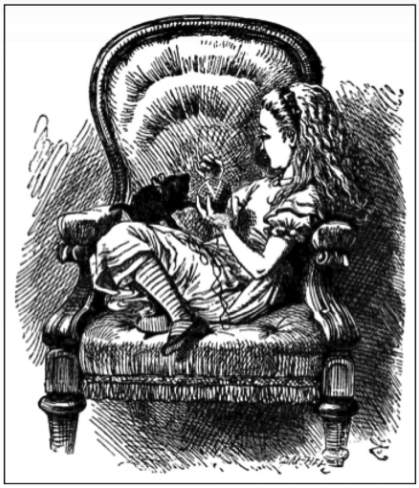
\includegraphics[width=0.9\textwidth]{Alice1}
\end{figure}
You can see Alice here playing with a ball of yarn and her kitten Dinah.
What I'd like you to imagine us doing here
is simplifying this image in different ways.
What we're going to do in particular is coarse-grain the image
in the following fashion. So, imagine dividing
this image up into grids, Figure \ref{fig:alice:coarse}, and then, at each grid point here –
if we were to zoom in to this digitized
version of Tenniel's image,
say just a little on Dinah's ear here –
we'll see a little patch of that image.

\begin{figure}[H]
	\caption{Coarse-graining Alice}\label{fig:alice:coarse}
	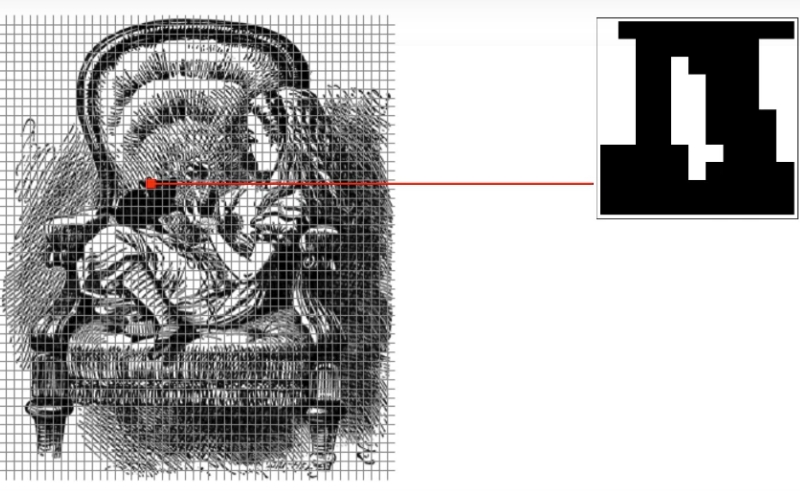
\includegraphics[width=0.9\textwidth]{Alice2}
\end{figure}
And what we're going to say
is for each of these patches,
we're going to represent them now.
Instead of all of the individual details –
the square is white, the square is black –
instead of all the individual details,
we're going to have that patch
just take a vote.
So that image, there it turns out
as majority black pixels,
and so it's going to coarse-grain
to a single chunky black pixel.
And we're going to go
grid square by grid square here,
taking all of the complexity
of the image within that ten by ten chunk
and compressing it down
to a single answer:
black or white, 1 or 0.
And if we go right next door
on that image,
here's a different part of Dinah,
different part of Alice's cat,
And what we can see in Figure \ref{fig:alice:voting}
is that even though this image patch
at the fine grain level is different,
the two descriptions in the different
parts of the image are different,
our course grading majority vote
will represent them identically.

\begin{figure}[H]
	\caption{Two different configuration coarse-grained identically.}\label{fig:alice:voting}
	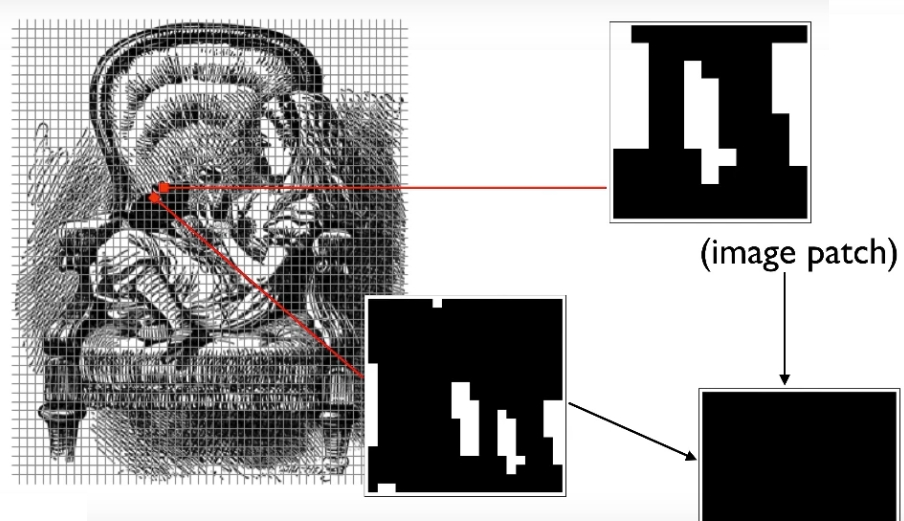
\includegraphics[width=0.9\textwidth]{Alice3}
\end{figure}
What we can see in Figure \ref{fig:alice:result:coarse:graining} is that on the left-hand side, we have the original image, and on the right-hand side
we have something that kind of looks pretty much like what
Alice sort of looks like, but we're missing quite a lot.

\begin{figure}[H]
	\caption{Majority coarse-graining.}\label{fig:alice:result:coarse:graining}
	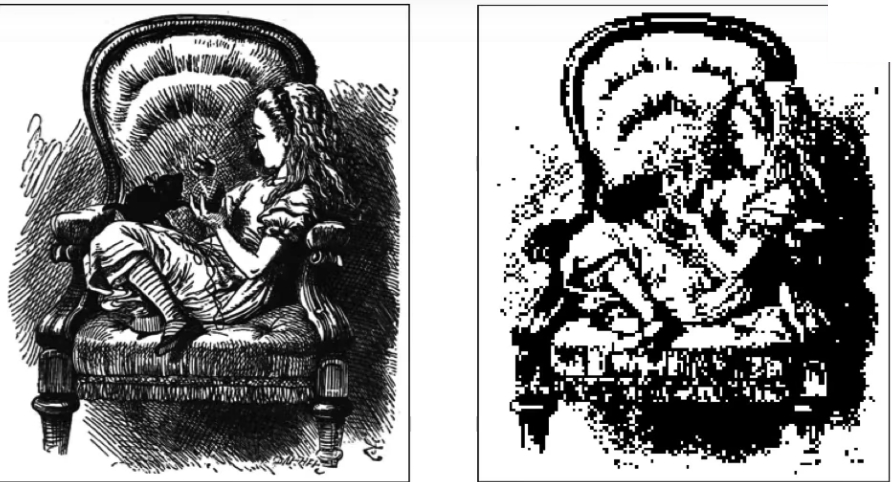
\includegraphics[width=0.9\textwidth]{Alice4}
\end{figure}

Here's another case, this is a different rule.
In this case, Figure \ref{fig:alice:result:decimation}, instead of taking the majority vote, I did what's called decimation,
at least in the literature, and this is a term that was invented
by the physicist Leo Kadanoff\cite{kadanoff2000statistical}
when he came to do this kind of coarse-graining, not on pictures
from ''Alice in Wonderland'', but on images of atoms
being spin up or spin down, and we'll talk about that
in a later module when we come to the Ising model.
\begin{figure}[H]
	\caption{Decimation.}\label{fig:alice:result:decimation}
	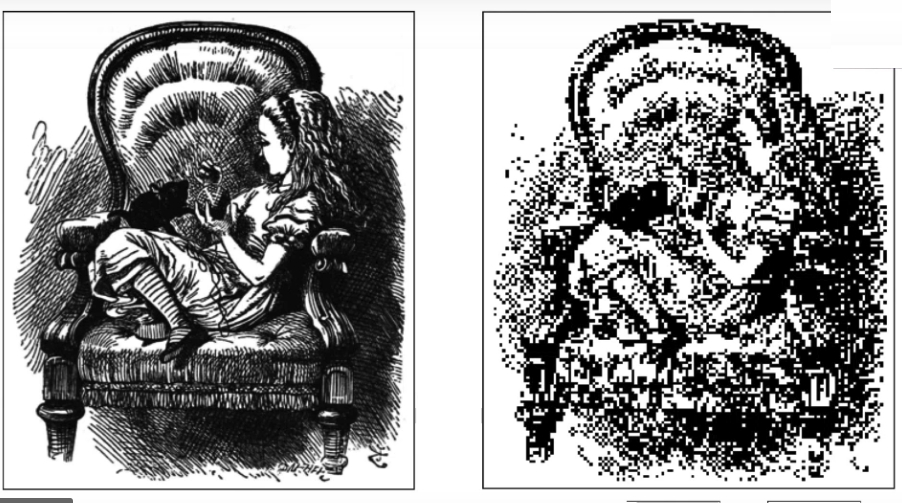
\includegraphics[width=0.9\textwidth]{Alice5}
\end{figure}

What Leo said to do is: Don't even bother to average over that grid square, just take the point in the top left corner,
and have that define it. You can see in this case here, if we use that decimation rule,
that same patch of die now gets mapped,
not to black, but to white.
So what I've introduced you to here
is two ways to simplify an image,
two ways to coarse-grain the image,
and, of course, different images
will now coarse-grain to the same thing.
I can make many microscopic changes
in Tenniel's original illustration,
and still get back
the same final image of Alice.
Of course, the microscopic changes
that my image is insensitive to,
or that, rather, my coarse-graining
of the image is insensitive to,
the microscopic changes will depend upon
the coarse-graining algorithm
that I choose.

So if I do the majority vote,
then I'll be able to make some changes
that won't show up,
and if I instead take
the decimation coarse-graining rule,
there's a different set of changes
that I can make at the microscopic level
that will leave the system unchanged.
When we come to compress images
in the real world,
we do this quite a lot.
So, when I took this the original image,
I actually had a perfect
representation of the image,
at least at that particular scale:
I had a tiff.
The file format there means
that every single pixel in the file
is registered as either being
on or off, black or white.
On the left-hand side,
you can see what happens
if I use my unfortunately non-patented
compression algorithm,
where here, instead of compressing it
using 10x10 grids,
I do a much less aggressive compression
where I only take little 3x3 grids.

\begin{figure}[h]
	\begin{center}
		\caption{Two coarse-graining schemes}\label{fig:alice:2:schemes}
		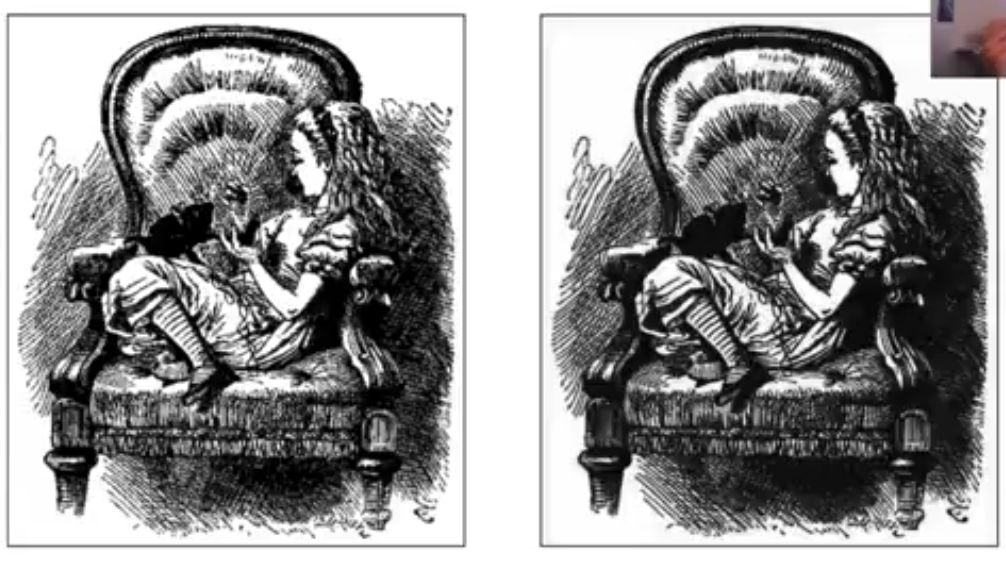
\includegraphics[width=0.8\textwidth]{Alice6}
	\end{center}
\end{figure}
If you compare how ugly
the 10x10 grid compression is,
to the 3x3 grid compression,
you might think,
''Hey, that's pretty good.''
And, in fact, by doing that,
by going from a grid that's 1x1,
by keeping track of every pixel,
and instead going to a grid that's 3x3,
I decreased the file size
by a factor of 9.
What I also can do is take that tiff file,
open it up, and max preview,
and now ask the computer
to do some coarse-graining for me.
because we spend a lot of time trying
to figure out how to compress images,
how to reduce their size,
how to throw away the information
that people don't need,
in order to allow the image
to be transmitted faster,
to be stored more conveniently.
So, on the right-hand side here--Figure \ref{fig:alice:2:schemes}--
we also have a coarse-graining of the Alice image, but now using a coarse-graining algorithm called the JPEG.
No one's ever referred to the JPEG as a coarse-graining algorithm, at least they don't do it that much.
What you can see is both images look reasonably good.
In fact, they have different properties,
so let's go zoom in here on Dinah.
What you can see on the left-hand side
is the majority vote coarse-graining.
One of the features of the majority vote
coarse-graining, by the way, you will see,
is that each pixel
is still a bit black or white.
If I zoom in again,
and I guess Dinah's looking here much more
like a rat now than she is like a cat,
but if you zoom in on Dinah
on the right-hand side,
you can see now the JPEG image
has made different choices
about what to keep and what to throw away.
Importantly, one of the ways
the JPEG works
is not in what we call real space,
in what the physicists call real space,
but instead what's called Fourian Space.
We'll talk a little bit more
about the distinction between
those two ways to represent an image,
but for now the simplest way
to think of it is this:
On the right-hand side,
what I did was I took the representation
of the image in the spatial field.
So, I took the entire array,
and I turned it by taking chunks
that were locally connected to each other.
I took little local chunks from the image,
and, for each of those chunks,
I did a little compression scheme.
I said all these differences here
don't matter,
you don't have to keep track
of all the either 9 or 100 pixels
within that square,

\begin{itemize}
	\item I'm going to summarize it,
	\item I'm going to coarse-grain it,
	\item I'm going to simplify it,
	\item I'm going to losslessly compress it –
\end{itemize}
all these words are equivalent,
different ways and different fields,
or rather different ways
that different fields
have discovered to talk about this –
I'm going to simplify all of those pixels
in a particular way.
On the right-hand side,
what the JPEG does is the following:
it does a transformation on this image,
it represents this image
in a very different way.
What it does is it represents the image
in terms of the fluctuations
that occur in it.
So, it takes the long-wavelength
parts of the image,
the fact that in the center
it's darker than it is around the edges,
and it puts that in one pixel.
Then it also takes
the high-frequency component,
the wiggles where the image is going
from black to white
very quickly along the line.
So, here, for example, you can see
on the back of the armchair
where Alice is sitting,
very fine grid lines.
What the JPEG does, is it says,
''There's a patch here where things
are oscillating very quickly,
so I'm going to put that over
in this high-frequency part
of the image data.''
It's also true of Alice's hair.
If you look at Alice's hair there,
she has these sort of kinky curls,
and those curls
have a high-frequency component
the JPEG records.
So, what the JPEG does is,
it represents that image now,
instead of representing it spatially –
so stuff on the left
is physically stuff that was on the left
in Tenniel's original recording –
it puts the low-frequency components
in one part
and the high-frequency components
in the other part.
And then it does two things.

\begin{itemize}
	\item First of all blurs them,
	so it does a kind of chunking
	coarse-graining on those components,
	\item and then also it just entirely cuts off
	all the high-frequency components
	in the image –
	because there are parts of that image
	that you yourself are not sensitive to,
	and those parts are where the image starts
	fluctuating back and forth very quickly.
\end{itemize}

In fact, you can see it:
on the right-hand side,
the JPEG looks smoother
than in the compression I've done.
In fact, what's so clever about the JPEG
is it actually respects the way
in which the human eye
records information.
Amazingly enough, of course,
when the human eyes
gets data from the real world,
and makes an image
on the back of your retina,
it appears almost like a set of pixels.
But before it actually wants to transmit
that image back into your brain
to make decisions,
it does itself
a series of coarse-grainings
using Gabor functions in the particular
sensitivity of the neurons.
It does a particular set
of coarse-grainings
that, in fact, the JPEG knows about.
So the things that your retina
is going to throw out anyway
as it transmits it backwards,
the JPEG has already thrown out
on your behalf.
\subsection{Coarse-graining part I - Clustering algorithms}

So, in the previous section,
you had an example of coarse-graining
from image compression
I showed you two different examples
of what you might call
real-space compression.
These were just things that
I made up,
that have some parallel
to what people have done
when they come to coarse-grain
a physical system.
What I did in particular
was take things
that were nearby each other in space.
I took a group
of objects, or a group of properties
of the system
that were nearby each other in space 
and I summarized them in some way.
So in the majority-rule case, for example,
all I did was, I took all the pixels
in a certain grid square, and I said, 
if the number of black pixels
outnumbers the number of white pixels,
then that pixel will be black,
and otherwise, it will be white.
And what I've done there, of course,
is taken a whole set of very different
grid squares, each of which
looks different,
and I mapped them all onto a single
kind of square
that only has one property, zero or one,
whereas here, in the ten-by-ten case,
there are in fact a hundred bits
of information, you might say.
So this is the general property
of coarse-graining; this is
a simple example of how we build
a function, $f$, that maps from some space $S$
to some space $S^\prime$.
This is a list of properties of, 
or this is the set of properties,
that describe the fine-grained system ---
for example, it could be the entire
productivity list,
the entire employment history
of every single person in the economy ---
and over here is a much,
usually much smaller set of quantities
that we're going to use to describe
the coarse-grained system.
Coarse-graining is something we do
all the time.
Sometimes, we make it up ahead of time.
So for example,
when we came to do the coarse-graining
of the image from Alice in Wonderland,
we just took a couple different ways
in which we thought
that simplifying the image
might work --- and of course,
what it means for it to work
is a problem that we often
don't think about 'til
right at the end, but here,
we took the majority vote.
We're saying,  look you know
if this pixel, if this kind of collection
of pixels here is mostly black,
let's just call it black.
And the idea is that your eye
might not really be
sensitive to it. In the end,
what we're doing when we choose
that rule is probably having a theory
about how the eye works,
or perhaps about what we care about
when we look at an image.
Of course, you'd be crazy to
do this on a bar code or QR code,
all right,
because in that case, the device
that's scanning the image
is much more sensitive
than your eye is,
and so if you took a photograph
of a QR code,
and then coarse-grained it
in the way we did,
the QR code would probably
no longer work.
In that case, the information that
we'd be throwing out,
the distinctions between the different
elements of this set here,
that the function all maps
to the same point here,
those distinctions would have been lost.
So sometimes,
we think about the problem we want
to solve,
and invent a coarse-graining algorithm.

Other times ---
and in fact this is becoming
increasingly common ---
other times, we don't know what
the coarse-graining is when we begin,
and in fact, we'll do something
really simple, like use
a clustering algorithm.

A classic example of clustering is k-means.
This takes a set of high-dimensional data, and because we can't afford
a high-dimensional whiteboard, we only have two,
so what I'm going to do here is,
I'm going to put a lot of
data points here, and maybe, for example,
this axis here is height,
and this axis here is weight, 
and these points here refer
to individuals of a species
that you've captured in the wild,
maybe these are birds, right.
And so what k-means will do is,
it will take that rich description,
where every individual is
described by a real number, 
on both the x and y axes here,
each bird you've caught, let's say,
has a certain height and a certain weight,
and you go out, and you sort of
laboriously, you know,
maybe you're in some tropical country,
like you're in Costa Rica or something,
which seems to be where
all the bird people go, 
and then you say, well, I don't know,
something's going on there,
and you hand it to k-means, which says,
oh, you know what, actually,
there's two clusters here, right?
There's this cluster, A,
and this cluster, B. And so
what k-means has done is
mapped from a two-dimensional
vector space, maybe not $R^2$
because you can't have, like, you know,
negative weights, so maybe it's just
the positive side of $R^2$, right,
it's mapped from that two-dimensional
vector space into a binary set, A and B.
So in general, when you call up
a clustering algorithm,
really what you're asking it to do
is coarse-grain my data, 
and then if you're a biologist,
you might be like, you know,
there's something funny, like
all the A birds, they're all female,
let's say, and all the B birds, 
they're all male, 
and now you feel really good
because in fact what you've done is,
you've discovered, using this data
here, using this rich high-dimensional
data, you've discovered a simple
low-dimensional explanation
for what's happening.
Why do birds have different weights?
Well, you know, the main thing is,
is if they're women, or if they're men,
if they're male or female.
So, clustering is sort of an automated way
to have the data suggest to you
what a good coarse-graining might be.
You may have noticed, of course, that
in fact, k-means operates with a notion
of closeness just as the
Alice in Wonderland coarse-graining did.
In both cases, we were saying that
things that were near each other, 
should probably be described by
a single description, right?
All these points here get
the description A; all these points here
get the description B.
k-means is in fact an example of
what we call a hard clustering, 
and in this case here it says that
each point is uniquely assigned
to a single cluster, and this kind of
hard clustering is a form of
coarse-graining, is the easiest to
understand, and we'll give an example of,
in particular, how hard clustering plays
a central role in information theory. OK.

There are other clustering algorithms
that give what are called soft clusterings,
and the most closely related
soft clustering algorithm to the
k-means one is called the GMM,
or the Gaussian mixture model.
And in fact the GMM is very similar
to k-means. What it does is, it takes
high-dimensional data, a vector of
high-dimensional data, or rather a set
of vectors of high-dimensional data,
right, each point referring to
a particular observation, and what the GMM
does is says, oh, you know, it looks like
this could be described as, like,
you're kind of drawing from two
Gaussians, right, the Gaussians
have a particular center, right,
they have a particular variance
and covariance matrix,
so they kind of, like,
these little sausages that lie here,
right,  and so what the GMM does is,
it produces a Bayesian model
of the way your data might have been
created,  and then for each point here,
it tells you the probability that that point
was drawn either from this Gaussian ---
we'll call that $G_1$ --- or this
Gaussian --- call it $G_2$.
So in fact, in this case, it's giving you
not a unique assignment, but it's
giving you a sort of probabilistic
assignment. In particular, it's mapping
this two-dimensional vector space ---
and let's say it finds two clusters ---
it's mapping that two-dimensional
vector space into the, sorry,
into the interval [0, 1], which you can
think of here as the probability
that the point was drawn from cluster A.
So this point here, right, really centered
to the first cluster, that would have a
very high probability of being a member
of $G_1$ and a much lower probability of
being a member of $G_2$.
So these are subtly different concepts
here --- there's the hard clustering case
when it takes each point and says, 
here is the coarse-grained category
you belong to. Just as in the case of the
Alice in Wonderland algorithm, what
we did was, we took that little
grid square, that ten-by-ten grid,
and we say,  you're majority zero,
therefore you belong to
the category zero, you're majority one,
you belong to the category one.
The soft clustering is a little weaker,
right; it sort of avoids
making a decision. You'll encounter,
probably in your own research,
different kinds of clustering algorithms,
different kinds of clustering choices.
People tend to prefer hard clustering,
because you don't have to think as hard
when you work with it.

\subsection{Coarse-graining part II - Entropy}

The last thing I promised you
was to tell you how coarse-graining
fit into the story of information theory.
So, even if you have not discovered
the information theory lectures,
you will get
a very brief introduction to it.

Let's imagine that we have some process,
let's say with 26 options:
there's the probability
that the process emits A,
the probability that the process emits B,
all the way down to the probability
that the process emits Z.

What information theory does,
one of the canonical questions
it asks, is:
How much information
is in that process?
This term also comes up:
How much entropy is in the process?
Another term is: How much uncertainty is in the process?

A process that has higher uncertainty –
in this case here, a process
when you stick your hand in the bag,
you don't know if you're going
to get an A or B or C
all the way down to Z –
a process that is more uncertain
has higher entropy,
and has higher information.

Claude Shannon invented a way
to measure, or to quantify,
to turn this big list of numbers,
this big list of probabilities,
into a single number which he then called
the uncertainty of the process itself.
He called that function H, the fundamental quantity
of information theory:

\begin{align*}
H \triangleq \sum p_i \log_2(p_i) \numberthis \label{eq:shannon:entropy}
\end{align*}

One of the questions you might have is: How did Shannon derive it?
What he did was, he came up with a series of axioms that he wanted this function to satisfy.

\begin{itemize}
	\item First of all, the maximum uncertainty that this distribution can have
	is if each of these probabilities is equally likely.
	So if the probability of A is 1 in 26, 	the probability of B is one in 26,
	and all the way down to Z, 	that should mean, if that's the case,
	you should be maximally uncertain 	about what's going to happen.
	That's the first thing he said.	The more uniform ... rather ...
	if it's perfectly uniform, 	the probabilities are perfectly uniform,
	that should be the condition of maximum uncertainty.
	\item He also wanted it to be symmetric,
	he didn't want it to discriminate
	between each of these different variables.
	So, for example,
	a probability distribution
	where A and B both had probability 0.5,
	and everything else was 0,
	should have the same uncertainty
	as the distribution where the probability
	of Y and Z are both 0.5,
	and everything else was 0.
	He didn't want to discriminate
	between the different options,
	and, for this reason, information theory
	is sometimes called a syntactic theory.
	So, well, that makes sense, right?
	If you shuffle these around,
	that should be good, right?
	It doesn't matter
	what these probabilities attach to.
	And the second thing
	is conditioned of maximal uncertainty.
	\item The coarse-graining axiom says the following: let's say you have three options, \{A,B,C\}.
	And, in this case here, for simplicity,
	we'll assume that these are independent
	in the sense that if I get an A,
	it doesn't affect
	what I'm going to get next;
	So, Shannon said, okay
	the entropy of that system
	should be equal given by (\ref{eq:coarse_grain_axiom}): the entropy of the coarse-grain system, plus the weighted entropies of those fine-grain distinctions.
\end{itemize}



\begin{align*}
H (P_A,P_B,P_C) = H(P_A,P_{B,C}) + (P_A+P_B)H(B,C) \numberthis \label{eq:coarse_grain_axiom}
\end{align*}
And once you demand
that this property here be obeyed, then you recover Shannon's
original formulation of entropy--(\ref{eq:shannon:entropy}). And it turns out
that this formulation is now unique: there is no other functional form
for how to convert a list of probabilities into a number describing uncertainty,
that obeys the condition of a maximum uncertainty, that obeys the syntax property
of being able to shuffle and get the same answer,
and that, finally, obeys Shannon's coarse-graining axiom. If you enforce all of those, this is the final formula that you're left with, no other formula will do.

And one of the very nice things about this
is that the coarse-graining axiom shows you how,
when you coarse-grain a system, the uncertainty,
the information that you have, goes down.
So let's say that instead of representing
the system like this \{A,B,C\},
I broke it up into these two pieces here, \{A,\{B,C\}\}
coarse-grained uncertainty,
and then a fine-grained uncertainty,
where I split the \{B,C\} case;
in that case, (\ref{eq:coarse_grain_axiom})  becomes (\ref{eq:coarse_grain}):
\begin{align*}
H (P_A,P_B,P_C) \ge& H(P_A,P_{B,C})  \numberthis \label{eq:coarse_grain}\\
H (P_A,P_B,P_C) >& H(P_A,P_{B,C})\text{, if there's some possibility of B and C}
\end{align*}

So, in this first module what have we done? I've given you a short introduction
to the idea of renormalization through the example of the microeconomics story. You have a microeconomic account of the world,
a very detailed description of what people are doing
that you then coarse-grain to a macroeconomic account.
That coarse-graining generally erases distinctions:
instead of distinguishing case B from case C,
you say, ''Ah, you know what? They're pretty much the same.''
We had an example of that coarse-graining property
in the case of coarse-graining the image of Alice in Wonderland.
And there, I actually gave you three examples,
majority rule coarse-graining, decimation coarse-graining,
and a more complicated, sort of Fourier space kind of coarse-graining,
called the JPEG, which of course is now in so much use
that your computer has a special chip that does JPEG decompression.
So, I gave you an example of how coarse-graining worked,
and, in this final part of the lecture of this first part of the module,
what I've done is tell you a little bit about
how coarse-graining plays a central role in information theory.

But coarse-graining is not enough. It's not enough
just to simplify the world, because, in the end, what scientists do
is something more than just create JPEGs. What a biologist does
is something more than just clustering – or rather you hope a biologist is doing
something more than just clustering, although you should check the literature
because sometimes they don't. And, in fact, many scientists
fall victim to this: they think that if you have a compressed,
efficient description of the world then you're done.

But you're not done, because what you want to do
with that compressed description is make predictions, produce explanations,
try to describe, but not just describe: try to explain what happened before
and what's going to happen next. And in order to do that,
you need a theory. And what renormalization does,
is it says, ''Great, congratulations, you've constructed a coarse-graining,
now, how is the theory connecting those different coarse-grained states,
how is that theory related to the one at the fundamental level?

How can you go, in other words, or rather what happens when you take
a full economic and psychological theory of the world
and coarse-grain it to macroeconomics? What happens when the macroeconomist
then tries to build a theory that relate his coarse-grain quantities?''
And so, in the next module, we will give you your first simple example
of how theories about the world change when the objects
that they describe simplify.

References: \cite{dedeo2018information,dedeo2013bootstrap,dedeo201716}

\section{Markov Chains}

\textit{This section is largely taken from the transcript.}

\subsection{Markov Chains}

So in the first module we gave you a series of examples about how as
scientists or indeed as engineers we try to simplify our observations. We don't
keep records of everything that happens at the finest possible detail. Instead
what we do very often is if we have some data at high resolution either out there
to be gathered or already on our hard drives, what we're often interested in
doing is simplifying it in some way and I give you a generic term for this which
we call coarse-graining.

In particular, what I did for the case of the etching
of Alice and her kitten Dinah is show you different coarse-graining
prescriptions, how you could take that image and strategically throw out
information, reduce the amount of
information you're keeping about the
original image and still if the coarse-
graining prescription is chosen well,
still keep some kind of sense of what's
happening in the system itself, what's
happening in this image, and so  maybe
you're not quite sure what kind of
animal Alice is playing with at this
point but at least you know that she's
playing with some kind of animal. We in
fact gave these three coarse-graining
prescriptions. The first one was majority
vote: I take a little square and I have
all the pixels vote on what color, black
or white, the output pixel should be and
in particular in the example here I took
a square that was 10 by 10 so I took a
hundred data points and just in the
majority vote assigned that either a 0
or 1 and made the pixel in other words
10 times larger and that's what happens
when you do it here. You could also do
something even simpler which is take
that 10 by 10 grid and just have the
pixel in the upper right-hand corner
sort of dictate what the final coarse-
grained pixel is going to be.

The final example I gave you we only talked about
it we didn't really show the mathematics
for how this happens was the compression
algorithm in actual use in the real
world and that's the JPEG. What the JPEG
does in fact is throw out information
that tells you about the very
fine scale oscillations in the data, the
patterns on the back of the armchair for
example and throw those out when it
thinks those are going to be
undetectable to the human eye while at
the same time keeping the overall longer
scale fluctuations in the image the
difference between let's say where the
light is and where the shadow is. It does
that through a Fourier transform and
essentially all it really does is just
chop off the high frequency components
in a way that engineers have decided is
at least not entirely visually unpleasing.

 So coarse-graining is
essential part of renormalization but it's
not the whole story in fact it's only
half, because as scientists what we do is
not just gather data and we don't just
simplify it. Instead what we do is we
tend to build models of that data so
let's take the highest resolution that
you can imagine for a particular system
and take the model that you think best
predicts or describes or explains the
data at that high resolution level. Then
we can ask the obvious question: What
model best describes or predicts or
explains the data at the coarse-grained
level and what's the relationship
between those two models the model that
describes everything and the model that
describes something. 

\begin{figure}[H]
	\caption{Commutation Diagram}\label{fig:commutation}
	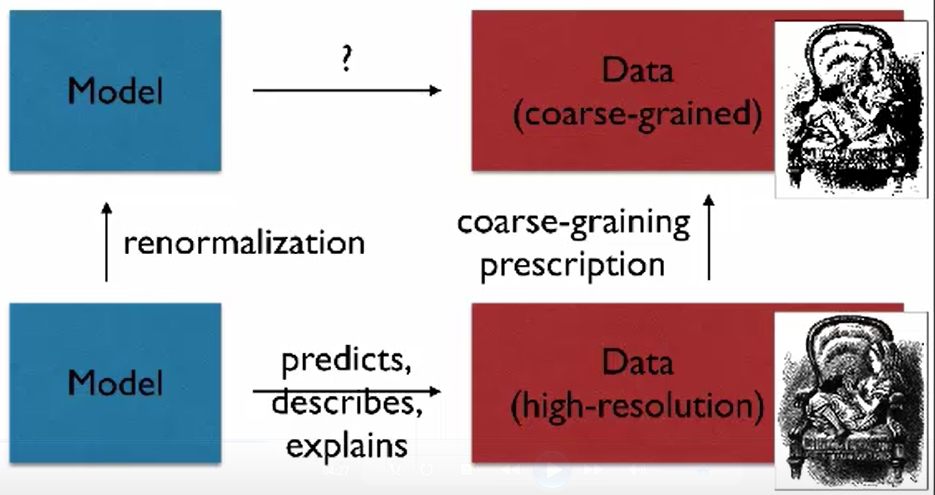
\includegraphics[width=0.9\textwidth]{commutation}
\end{figure}

The entire story of renormalization, Figure \ref{fig:commutation}, is the relationship between what happens when you coarse-grain the data and what happens
when you look at the underlying structures of the models that that
coarse-graining demands. Surprisingly as
we'll see sometimes when you coarse-grain the data the models that you need
get more complicated. Sometimes
conversely they simplify and it'll be
that kind of process that we'll study
now. In order to describe the
normalization you'll see of course that
I have to tell you not just what is
happening to the data but also what's
happening to the model so I have to give
you an example not just of some data
that we're coarse-graining but of a model
that describes it.

The model that we'll use is the Markov
chain. So how do Markov chains work, what
do they operate on, what are they
supposed to describe or explain or
predict? In general Markov chains
describe time series, a series of
observations that unfold that
evolve or unfold one moment after
another. The simplest case is when each
observation is a symbolic unit so you
know an A or B or C, when the stock
went up or the stock went down, that the
person said this word or that word.

A more complicated story is that each of
those observations could be a continuous
number like a temperature or a field the
value of let's say of the electric field
at a certain point in time at a certain
point in space. Here we'll just deal with
symbolic time series because they're
much easier to handle at least when the
number of symbols is small. So that's our
basic idea that's our fine-grained data
and then we're going to imagine coarse-
graining that to produce a lower
resolution time series. Now of course
that's not the only way to coarse-grain
a time series. You could also imagine
coarse-graining each symbol so let's say
each point in time you chose from a set
of 10 symbols. One way to coarse-grain
that time series is instead of choosing
from a set of 10 you map those 10
symbols to either a symbol A or a symbol
B that kind of coarse-graining something
we'll see a little bit later you might
think of it as a projection you're
projecting down the state space.

Here we'll do something a little simpler.
Imagine for example the time series was
gathered at intervals of one second.
Now what we're going to imagine is that
you know you didn't have expensive
enough equipment or your hard drive got
full so instead of keeping every second
of the evolution instead what you did
was let's say kept every other second or
every third second. In other words you
took a block of the time series and you
decimated it. You just took the first
observation within each block over time
sort of a one-dimensional version of how
we coarse-grained the sketch of Alice by
John Tenniel. All right so that's the
data we'll be operating on. The Markov
chain provides you a model of how our
time series is produced and then what
we're going to see is what happens to
those models as you ask them to describe
or predict or explain
the lower resolution version. We'll
compare one model to another as they
operate on different kinds of data.

Figure \ref{fig:markov1} represents a Markov chain. On the left-hand
side what I've shown you is a depiction of the model I'll tell you how to read
the representation in a second. On the right hand side there's a sample bit of
data that it might predict or explain. In this case what I did was I just ran the
model itself because it's a nice way it's a generative one it will tell you what's
going to happen next and so I can just start somewhere and allow the model to
produce a simulated time series.

\begin{figure}[H]
	\caption{Markov Chain: deterministic emission of symbols}\label{fig:markov1}
	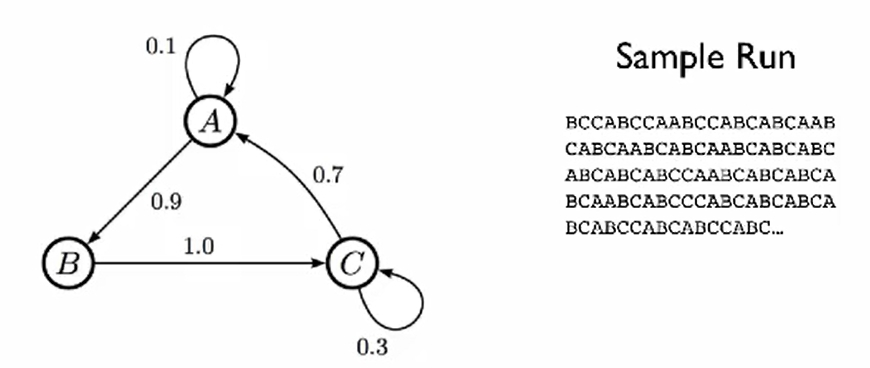
\includegraphics[width=0.9\textwidth]{markov1}
\end{figure}

Markov chains are stochastic so in any
particular case it will produce
generically a different sample run. On
the right-hand side what you have is
just one example of the kind of data a
Markov chain could produce, conversely
the kind of data that a Markov chain
could describe or predict. So the
left-hand side shows the Markov chain
itself. What you see there are three
nodes A, B and C and it's simple enough
when the system is in state A it emits
the symbol A when it's in state B it
emits the symbol B and when it's the
state C it emits the symbol C and then
upon emitting that symbol it makes a
transition. It jumps to one of the other
states and the probability of jumping to
each of those other states is dictated
by the model itself and in fact I
represented that here by the arrows. So
let's say you begin in state A. With 90
percent probability you jump to state B.
Say you're in state C, with 30 percent
probability you stay in state C, with 70
percent probability you jump to state A.
Specifying those transition
probabilities corresponds to specifying
the entire set of free parameters for
the Markov chain. Once you tell me the
transition probabilities you've told me
everything I need to know about the
underlying model.

Markov chains are fun
but it's also important to realize how
limited they are. For example if I am at
the B and then I'm at the C what happens
next does not depend upon the fact that I
emitted a B. When I'm in state C it
doesn't matter how I got there. Similarly
if I'm in state A it doesn't matter how
I got there. Whatever I do is conditioned
entirely upon what's happening at the
current time step. There's no nonlocality
in the Markov chain is another way to
put it or you can think of it as a
system with no memory. If I'm in state B
that defines everything about what's
going to happen next.
And so you can see how to read this
sample run. In the sample run I begin
in state B and in fact deterministically
I know it has to happen next and go to
state C. In the sample run when I ran
this Markov chain forward it chose
randomly to stay in state C which will
happen 30\% of the time so it emitted
symbol B and C then it stayed in C and
then in fact on the next time step to
jump to A and you can see that system as
it evolved from one moment to the next.

So now let's take the observable data
associated with that Markov chain or one
instantiation of that data associated
the Markov chain and coarse-grain it
using this decimation transformation and
in particular what I'm going to do is
just take blocks of two observations in
a row and take out the second one or
conversely I'm going to coarse-grain
that block of two observations to a
single observation and I'll have it
dictated by the value of the first point
in that block. So in this case I've used
blocks of size 2. I have coarse-grained the
data at let's say a two-second time
scale. It's easy enough to build the
Markov chain associated with that
coarse-grain run and in particular let's just
walk through Figure \ref{fig:markov2} to
see that the arrows make sense.

\begin{figure}[H]
	\caption{Coarse-grained Markov Chain}\label{fig:markov2}
	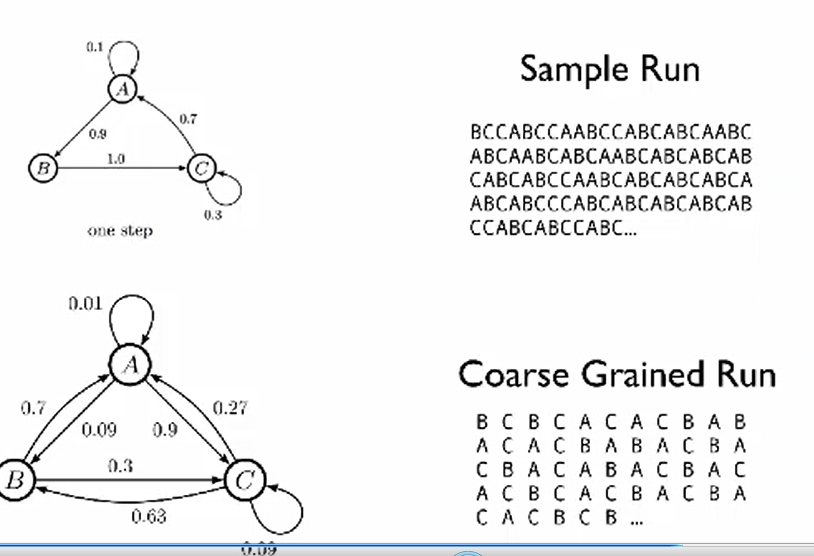
\includegraphics[width=0.9\textwidth]{markov2}
\end{figure}

 In the
next section I'll tell you how to derive
these mathematically but for now it's a
useful exercise to see if we can
understand the relationship between the
one step in the two step model.
Notice that in the one step model it's
impossible for the system to jump from B
to A. But in fact in the coarse-grained
system it's in fact very likely that if
you see a B the next symbol you'll see
will be an A. It happens 70 percent of
the time and you can see if you look at
the coarse-grained run it's pretty easy to
find cases where you have B and then A.
In fact, on the first line I see it once
and on the second line I see it three
times BA BA CB A. But in the sample right
at the finer grain time scale that's
impossible and of course that's
impossible because when you're in state B
you deterministically go to state C. At the
coarse-grained timescale though it's
pretty easy to go from B to A. You go by
AC but that C step is of course
unobservable. It's coarse-grained away.
And in fact in that case if you start in
state B 100\% of the time you go to state
C. And so for it to show up as an A at
the next time step all that has to
happen is that when you're in state C
you have to jump to A and that happens 70
percent of the time. And so what I've
done there in a sort of laborious way is
tell you exactly why the arrow from B to
A is labeled with a 70\% probability. Of
course that's just when you coarse-grade
from the fine-grained time scale to
blocks of two you can just as easily
imagine coarse-graining that
system from blocks up to two blocks of
three, to blocks of four and so forth
and so if we look here and how this
model evolves over time we're basically
telling the parallel story to how the
data is being coarse-grained we coarse-
grain in blocks of two steps or we coarse-
grain in blocks of three steps. As you
can see the model changes and it's a
little bit hard if you look at it to see
exactly the logic of that change. When
you go from one step to two step in some
senses the model maybe looks like it
gets a bit more complicated. All I mean
is that there are some transitions that
now become possible that were impossible
before. You become a little less certain
about what's going to happen. Except then
when I go to three steps, Figure \ref{fig:markov3}, some of those
transitions go away again so in fact
I become a little bit more certain
now. 

\begin{figure}[H]
	\caption{Even more coarse-grained Markov Chain}\label{fig:markov3}
	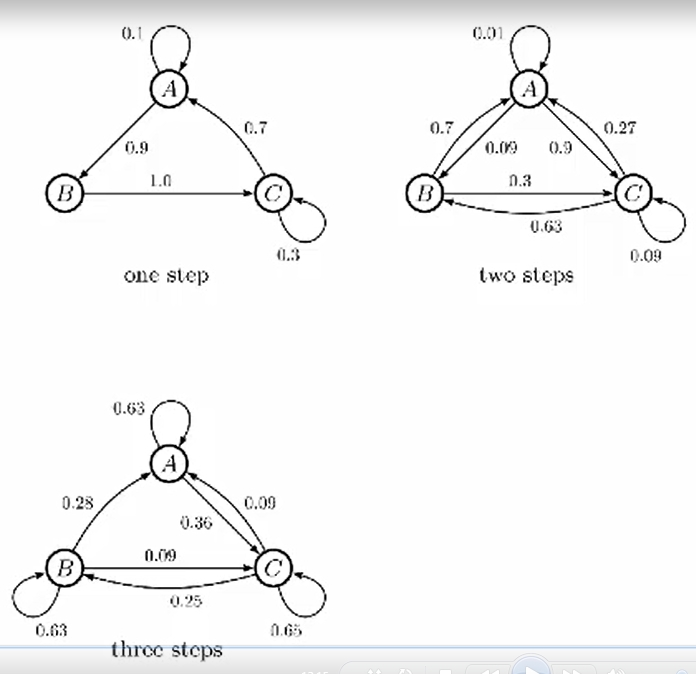
\includegraphics[width=0.9\textwidth]{markov3}
\end{figure}

So what is the limit of this process?
What happens when we start coarse-
graining not on the two step but with a
three step time scale, when we continue
this and coarse-grain on increasingly
longer and longer time scales? It turns
out that models tend to flow to what
we'll call fixed points. In other words
as you go from one coarse-graining level
to the next, the corresponding model
tends to change less and less, at least
if you wait long enough. They tend to
converge on a single model as the coarse-
graining timescale gets longer and
longer and longer. And in fact not only
does every Markov chain converge to a
particular sort of limit case
Markov chain. In fact the Markov chains
that the Markov chain that it
converges to has a particularly simple
structure. Here it is. Here's the limit
point. If you take that one step Markov
chain and ask what happens if you coarse-
grain the data on really long time
scales. If you look at the transition
probabilities
you'll notice that every state has
incoming arrows all with the same weight.
The chance of going to a C is
independent upon which state you were in
previously. It's always in this limit
it's always 40\%. Similarly if
you're transitioning to state A it
doesn't matter where you come from. The
probability is always the same
31 percent. If you think about how many
parameters you need to describe the
model at the one-step case, well, you have
three states, each state has three
transition probabilities but since
probabilities have to sum to one in fact
for each state you only have two free
parameters. So you have three states, two
free parameters each. There's six
parameters that describe an arbitrary
Markov model on three states. However, if
the pattern holds and it does for nearly
every Markov chain that you can write
down. Not everyone just nearly everyone.
But if that pattern holds what that
means is that when you coarse-grain on
sufficiently long time scales you only
in fact need two parameters. It's a
remarkable compression. In other words
not just of the data but of the model
space. You begin in this sort of six
dimensional manifold but if you coarse-
grain the data enough the models
corresponding to that coarse-graining all
flow to this very low-dimensional, two-
dimensional in fact, manifold,
where the model is described simply by
the incoming probabilities to each of
those three states and since they all
have to be the same the chance of you
going to C is the same no matter where
you begin and the chance of you going B
be is the same no matter where you begin
and since the probabilities outgoing
from each state have to be one even
though there are three probabilities to
specify only two of them are needed. The
third one is just one minus
the sum of the other two.

In the next module
I'll show you how to make
these computations exact
but for now this is our first
example of how theories change when the
data you ask them to describe is
coarse-grained.

\subsection{Mathematics of coarse-grained Markov chains}

In the previous module,
I gave you a cartoon example
of how a Markov chain coarse-grains
as you go to longer
and longer time blocks.
So, I gave you a Markov chain
that worked, let’s say,
at one second resolution,
and then I showed you
how to build a Markov chain
that worked if your time
resolution was poor.
So, for example let’s say,
you could only observe the first second
of each two second block.
That decimation coarse-graining
transforms the underlying model itself,
and so, as you saw,
when we went from the fine-grained model,
Markov chain,
and coarse-grained it
on blocks of scale 2,
that Markov chain seemed to get
a little more complicated,
and all I mean by that,
it seemed to have more arrows –
we don’t really have good way
to judge the complexity of a Markov chain.
But the model certainly changed,
and it didn't necessarily
change for the better.
Even though we simplified
our observations,
the model itself seemed to do something,
well, not necessarily weird,
but something that didn't seem to have
a particular structure to how it changed.
But if we coarse-grained
on sufficiently long timescales,
it appeared that the Markov chain
coarse-grained to a simpler case
where the outgoing probabilities
for each of the states were the same.
So, each state had the same probability
to go to state A, B, C, and D
as the other states did.

In this module, here, what I’m going to do
is show you how to do
a little bit of linear algebra
to actually make that concept rigorous,
to talk about how a Markov
chain will, eventually,
if you coarse-grain enough,
simplify into a small into a smaller
subspace of all possible models.
This would be one of our first examples
of a renormalization group transformation
that takes you
to what we call a fixed point.
So, what I’m going to do
is give you that example
using a much simpler Markov chain
which I’ve drawn on the board here.
This Markov chain has two states, A and B.
What I’ve done,
instead of writing
exact numerical probabilities
for each of these transitions,
I’ve just parameterized the system
with one parameter $\epsilon$.

So, in this case here,
what we have is a system
that can jump from A to B
with probability $1-\epsilon$,
or it can stay in state A
with probability $\epsilon$.
If we make $\epsilon$ small,
that means that the probability
to stay in state A is small,
so the system will tend
to oscillate back and forth –
it will go ABABAB.
As $\epsilon$ gets larger and larger,
it will have a certain probability
to stay in state A.
So, it might it might, in fact,
go AAABBBABAABB,
it’s a kind of slippy counter
as $\epsilon$ gets larger and larger.
So, a simple way
to write or describe this model
is to imagine that we describe
the state of the system
using your column vector.
In this case the column vector
will have two entries:
the first entry will be the probability
that you’re in state A;
the second entry will be the probability
that you’re in state B.
Now we can describe
the evolution of that system over time
using a two-by-two matrix
where the entries of the matrix
look like this.

Each term here
is a conditional probability
that tells you how you move
depending upon which state you’re in.
So, for example, we can see
if the matrix is written like this,
where, for example, the first term
in the top-left corner here of this matrix
is the probability
that given you’re in state A,
what’s the probability
that you transition to state A,
stay in state A.
Or here, for example,
if you’re in the top-right corner,
this is the probability that,
given you’re in state B,
you transition to state A.
Notice that when you do
the matrix multiplication here,
and I’ll just do the top one
to give you a sense of how this works,
in case you haven’t seen it before,
This top entry here now says
that the probability
that you’re in state A
after one time step
is the probability
that you begin in state A
and transition to the same state A,
you stay in that state,
the probability of A given A,
plus the probability
that if you begin in state B,
the probability of state B,
times the probability
of transitioning from B to A.
And then we’ll leave as a homework example
for you to compute the second term here.
So what we see is we can now
evolve the system through time
by multiplying using this matrix here,
which is sometimes called
stochastic matrix.
One of the things
that you can see right away
that makes this matrix special
compared to all two-by-two matrices
is that all the columns here
have to sum to 1.
If you’re in state A,
one of two things
in this case must happen.
You either stay in the state
or you transition to another state.
There’s no other possibilities,
and the probabilities therefore exhaust
the space and have to sum to 1.
Another feature, of course,
of a stochastic matrix
is none of these entries can be negative.
So stochastic matrices are
an interesting sort of subspace
of all the possible two-by-two matrices
that you will encounter in your life.
Once you’ve represented the Markov chain
as a stochastic matrix,
and I’ll write a particular Markov chain
that we have here in this new form,
it becomes a simple matter
to talk about what happens
if you skip observations.
If the system jumps 2 time-steps
before you see it again,
all I do is take this evolution matrix T –
sometimes we call it an evolution operator
if we’re feeling a little punchy –
all we do is take
this evolution operator T
and multiply it by itself.
And now what we have
is when this matrix
acts on a probability vector
it takes it one step in the future.
You act on that matrix again
on the results of that,
and it takes you two steps in the future.
And so the Markov chain corresponding
to the observation series
that’s been coarse-grained
in blocks of two,
and this is decimation course graining
where we take the first observation,
we can now write that very simply
as the product of this matrix with itself.
So I'll write that out for you,
and just show you how the first term goes.
The probability that if you’re in state A,
and you stay in state A two steps later,
is equal to this product here:
$\epsilon*2 + (1-\epsilon)^2$
And we’ll leave these other entries
as an exercise, as you please.
In words what this says
is the probability
that if you begin in state A,
you’ll be in state A two steps later,
is the sum of two possibilities:
the first is, of course,
if you stay in the state A –
if you just stay in the state A
on the second time-step,
or on the first time-step
and the second time-step.
So the probability
of that happening is $\epsilon^2$,
the probability that you stay in A twice;
or the other possibility
is that you start in state A
on the second time-step
you jump to state B,
and then you quickly jump back
to state A before anybody notices.
And that’s the second term here $(1-\epsilon)^2$.
So now we can see that in some sense
it’s a rather trivial problem
to see what happens to this matrix
as you continue to coarse-grain:
if you take blocks of 3, 4, or 5,
all you have to do
to see the resulting model
is raise T to the power
that you’re interested in.
Here n is now just the block size.

\subsection{Mathematics of coarse-grained Markov Chains: The General Case }

So, can we say anything
general about that process?
The answer turns out to be: Yes.
And what we're going to do
is represent this matrix
not in the form
that you're familiar with
the $\epsilon$ and $1-\epsilon$ form
where the column vector refers to
the probability of being in state A
or the probability of being in state B
instead what we're going to do is
diagonalize this matrix
so if the matrix is T what we're
going to do is find its eigenvectors
and the eigenvectors
of the matrix T are defined
by T acting on let's say
the first eigenvector
gives you back the first eigenvector
potentially times some constant $\lambda$,
so this is the eigenvector
of the transition matrix or
the evolution operator T
and this is the eigenvalue.

A matrix like this generically has two
eigenvectors
and two
eigenvalues
and so we can write the eigenvectors
as $v_1$ and $v_2$.

And now what i'm going to do is for an arbitrary
probability distribution over states
A and B. I'm going to represent that
as a sum,
as a weighted sum over these two eigenvectors,
so we'll call that $a_1v_1 + a_2v_2$.
And so if I now make a column vector
that represents that probability
in eigenvector space
what I'll have is an $a_1$ and $a_2$ like this.
So if I have diagonalized
that matrix now
when it acts upon
this transform space
it looks it takes a very simple form,
and in fact, I'll write out
the exact form it takes here
the matrix now become diagonal
and when it acts
on the diagonalized version
of the probability vector
as you would expect
given the nature of
the eigenvectors itself
It turns into
a scaled version of
each of these two entries.
So what I've done here is go from
this way of representing
the Markov chain
to this diagonalized representation here
which we can call T hat
and T hat now acts not on the
probability of being in states A and B
but instead on the amount
of probability that you have
in the first eigenvector pattern
and the amount of probability you have
in the second eigenvector pattern.
What you can see here is that this matrix,
the two eigenvalues it has,
one of these eigenvalues is equal to 1.
And in fact it turns out from a theory
that you can prove in linear algebra
that any stochastic matrix
will have as its largest eigenvalue
something whose
absolute value is equal to 1.

In fact sometimes this eigenvalue here
can be negative one.
Sometimes it can even be imaginary.
Generically for most ordinary
stochastic matrices
including the one we're going to look at here
and the conditions on that
are somewhat technical
we have to have irreducibility [or] ergodicity,
but in general what you'll have
is that the largest eigenvalue
for stochastic matrix is equal to unity.
All the other eigenvalues
will have absolute values
that are smaller than 1.
So notice here as long as $\epsilon$
 is less than unity
right, as long as there's some probability
for a transition between A and B
this term here will have
an absolute value less than 1.
Notice that if $\epsilon<\frac{1}{2}$ in fact
the second eigenvalue will be negative,
but it still in its absolute value
will be less than 1.
So now we've reduced the problem
of taking $T^N$
to the problem of taking $\widehat{T}^N$ to the N
where $\widehat{T}$ is 1 on the diagonal
and then $2\epsilon-1$ here
and that is now acting
on this transformed representation of the
probabilities of being in state A and B.
If we raise this here to the power of N
this matrix takes a very simple form,
this first diagonal term
of course $1^n$ 1
the off diagonal terms remain 0
and now you have $(2\epsilon-1)^n$ 
again acting on
the transformed representation.
As n gets very large this term here
because it is less than 1 and
absolute value
will continue to get smaller and smaller
so for example let's take
the simple case 2
where $\epsilon$ is equal to let's say $\frac{1}{den}$.

In that case along the diagonal
you'll have
a 1 up here and a negative $\frac{1}{den}$ to the n here
and when you act upon an
arbitrary column vector $a_1 a_2$
this will turn into $a_1$
will remain unchanged
but $a_2$ will be down by a very large factor
so let's say if n is a thousand
then $\frac{1}{2}^n$
is down by a factor of a million or so.
There will be this minus sign here
So depending upon whether n is even or odd
it will be a very tiny positive number
or a very tiny negative number
but in general as you take
increasingly large powers of this T
You will find that no matter what
you put into the system,
no matter what combination
of $a_1 a_2$ you put into the system
out the other side you will
get a vector that is pure $a_1$.
Another way to say this
using the language of the probability
of being in each of these states
is that if you
coarse-grain your data enough
the corresponding model will take
any probability distribution
and map it directly to that first
eigenvector of the system.
That first eigenvector has a special name.
It's called the stationary distribution.
It's called the stationary distribution
of the original stochastic matrix.
And so now
we know that no matter
what you put in.
Let's say if you begin entirely in state A
if the system has been coarse-grained enough,
after one coarse-grain time step
using the evolution operator $T^2$
or rather$T^n$ as n gets very large.
At the next time step you will go to a unique
probability distribution given by $v_1$
and in fact if you begin in state B,
you will also be taken
to the identical
probability distribution  $v_1$.
And so in the end
the matrix will take the following form.
If you begin in state A
you have some probability called P(A)
of staying in state A.
And you have some probability of ending up and state B
called P(B) and then we know, of course,
that that's equal to 1 - P(A)
Similarly, if you're in state B
you have some probability
to stay in state B
and you have some probability
to end up back in state A
and, again, we can write
the probability of being in state B
as 1 minus the probability
of being in state A
so
What the simplification means
is that no matter
what probabilities
for transitions you put in here
and in particular we are free
at short time scales to put arbitrary
probabilities for the self loop
for A and arbitrary probabilities
for the self loop for B.
If you begin with this description on short time scales,
if you renormalize enough,
if you coarse-grain the observations enough
and ask what the corresponding model is
you find in fact that every model can be
described by a single parameter P(A).
You move from models
that exist in a 2-dimensional space
where I have to tell you the self-loop
probabilities for each of these individual states.
If you coarse-grain enough that takes you
to a set of models that can be described
by a single probability, P(A)
and so in fact one way to imagine the
limit of this coarse-graining process
how all of these different Markov chains
flow is in a following diagram
which we call, sometimes call,
phase diagram for this system,
which I can draw like this.
On the X axis we have
the self-loop probability for the A state
and on the y-axis we have
the self-loop probability for the B state
So every point in this space
refers to a distinct Markov chain model.
All of these models actually flow
to a single line on this plane.
All the points on this line here
have the potential to be fixed points
that as you coarse-grain the system
further and further
they all end up on this line
where the probability
of the self-loop for the A state is equal
to 1 minus the probability
for the self-loop for the B state
and the way to think about this is P(A) given A
when you coarse-grain enough
just becomes the stationary probability,
the stationary distribution for that Markov chain P(A)
the self-loop probability for B
just becomes the probability for B.
And we know that that now
has to be equal to 1 - P(A)
for that stationary distribution.
So what we find is that as you
continue to renormalize this system
as you continue to coarse-grain
and ask what the corresponding model is
you get driven towards this line here
and as you get driven to that line here
you flow to some
what we call fixed point
where you get closer and closer
to the limit of T to the n
as n goes to infinity.
So that's a more formal, still somewhat
cartoonish story that I've told
the reason I say it's cartoonish is that
I haven't told you the exact conditions
for this flow to work.
Implicitly what you have to have
is that first eigenvalue
has to be equal to one and there
can be no other eigenvalues
that also have
absolute value equal to one.
So for example a model that does not flow
model that does not flow
to somewhere on this line
is one where the system
continually oscillates back and forth.
In that case the self-loop probability for A is zero,
the self-loop probability for B is zero.
But no matter how many times
you multiply the system by itself
it never kind of blurs out
and gives you a stationary distribution.
I haven't told you the exact conditions
that tell you that some
of these models are ruled out
sort of on the corners of this space.
But basically if you're somewhere in the interior
you always flow to a unique fixed point
under the coarse-graining operation.

\subsection{A puzzle: origin of the slippy counter}

So, in the previous section of this module
we delve a little bit deeper into the mathematics
of how transition matrices like these
renormalize when you coarse-grain the data,
what does the accompanying model do.
And what we found is a kind of phase diagram here
for the transition matricies
and in fact what I've done is produced a general phase diagram
that's good for any two-state Markov chain.
And what we find is that in general,
modulo some slightly tricky
things to do with the case
where the first eigenvalue is imaginary,
but modulo these kind of tricky cases,
if you begin with a model anywhere in this space
you eventually flow to some point on
this diagonal line here
and on that diagonal line every update you do
no matter where you begin
no matter what your initial distribution is
one update will take you directly
to the stationary distribution which is
now defined not by two parameters,
but in fact by only one,
you go from a two-dimensional manifold
down to a one-dimensional manifold
and stay there.
You don't flow once you hit this line.
You don't kind of move back or forth.
It's sort of a line of fixed points
for this renormalization transformation.
So, in this final section,
somewhat optional,
I'd like to ask kind of fun question.

So, we begin at this point here
and let's take this matrix here where
the Epsilon's are equal to each other,
they lie somewhere along that line,
where the self-loop probability for A
is equal to the self-loop probability for B.
What happened or where
did that matrix come from?
Is it possible to find another matrix
that works at a finer time scale
than you thought could have
been there in the first place?
Another way to think of this is that
you've gathered some data
in order to get this model here.
But what if you were gathering
the data not rapidly enough
to hit the actual sort of fundamental clock of the system.
What if in fact your data was already
coarse-grained and you could imagine this?
Imagine that you built this model
here off of some data,
then your collaborator calls you up
and say: I got great news,
we have this new high resolution
time-sensing device
that enables us to actually measure not
every 10 minutes, but in fact every minute
Well great, okay, what kind of model
could T have been generated by?
The mathematical way to answer this
question or to ask this question
is to say can we find a transition matrix A
such that when you square it you get the transition matrix T,
and this is under the assumption that your collaborator has come up
with a resolution device now that can split
twice as fast as it originally could.
So let's find it. Let's assume T
is given by this matrix form here
and then all we have to do is figure out
All we have to do now is figure out
what A and B are in this new transition matrix here.
We have to square this matrix,
set it equal to T and solve for A and B
and in fact I'll write this
in a slightly better fashion
so that A and B become
the self-loop probabilities
for the two states.
So, our challenge becomes
find A and B.
Okay, let's do it.
Here is our problem. We're going to
square A or multiply A by itself.
And we're going to set that equal
at the end to the transition matrix T.
So if we do that multiplication
we find in the top corner here
we have $a^2_1-B(1-1)$
And let's say down to the right
we have ''a'' times ''1 - b'' plus ''b'' times ''1 - b''.
Down here we have
''a'' times ''1 - a'' plus ''b'' times ''1 - a''
and in the far lower right-hand corner
we have
''1 - a'' times ''1 - b'' plus ''b'' squared.
This we're going to set equal to our original
and much-beloved transition matrix T.

So
We'll leave the full solution
to the homework,
but I'll give you a little clue on how to do it
which is that in fact A and B have to be equal.
If A and B were not equal
we wouldn't be able to satisfy
this set of equations here.
And so once I tell you that A and B
are equal, then I can say

Ok, let's try and solve
part of this problem
by setting that term there equal to $\epsilon$.
So, what happens we have a squared
plus 1 minus a squared
because I've told you that ''a'' is equal to ''b'',
you can prove it yourself if you're going
to be distressed by what is about to happen.
So I have $a^2 + (1-a)^2$ so that's
$a^2_1-2a+a^2=\epsilon$

Using my amazing algebra skills we have
$2a^2-2a+(1-\epsilon)  = 0$

And now we use our quadratic equation
skills to solve for a.
We have negative b plus or minus
root b squared that's 4
minus 4 times a times c
which is one minus epsilon all over
2 times the square term coefficient
which is four.
If I simplify that I get one half plus or minus
And now I can pull out the factor of two here
So we have one half square root one minus
$2(1-\epsilon)$.
Okay, so far so good.

What I'd like you to notice is what
happens when let's say $\epsilon=\frac{1}{4}$.
In this case under the square root sign here
we have the square root of one minus two
times three over four which is equal to
one minus three over two which is
equal to minus one half
in other words the only way to satisfy
the equation $S^2=T$
is if some of the components of this matrix here
have imaginary or generally complex entries.
But if A has complex entries then it
corresponds or rather cannot correspond to any
natural stochastic matrix because we
interpret the entries of A
in fact as transition probabilities, and now we're
being asked to imagine
that some of those transition probabilities are equal to things
like $\frac{1}{2} \pm \frac{1}{2} \sqrt{-\frac{1}{2}}$
So in fact what we found is that T is not
or rather when epsilon is in fact as you can work out
when epsilon is less than 1/2
that matrix T could not have been generated by a
coarse-graining of any finer scaled two-state system.
So where did T come from?
Well, one way to see where the problem is is the following.
If we imagine that the state or the system
is a good counter
so that it oscillates ABABABAB
and only very rarely slips and produces a BB
or AA or even more rarely a
triple A or triple B
If it's a good counter meaning epsilon is small
What would this look like if we expanded it
at the finer timescale?
In that case we'd have A ? B ? A ? B ? A
and we'd have to fill in this gap here.
But if we only had two states,
if we only had the possibility of it filling in
with either A or B
let's imagine for example
we filled that question mark at that point with A.
In that case at time $t_1$
the system was in state A
and jumped directly to A
and then at time t plus $\frac{1}{2}$
the finer timescale, it jumped from state A
directly to state B.
But if it's doing this deterministically,
then how can it know that at this time step
it's in A and should jump to A
and at this time step or at this time step here
it's an A again,
but this time it should jump to B?
Markov chains are memoryless, the only thing that
determines what a Markov chain will do next
is the state that it happens to be in.
And again, you can imagine filling this state in here with B.
And now you have the same problem,
because here the state goes from A
jumps to B, very good.
Okay, here the state goes to B,
from B it jumps to B, okay good.
Now if the state deterministically jumps from B to B,
we know this one here has to be B.
But then we have a problem because we have to explain
how the system somehow knows that
this B is different from the last B?
How the system knows that okay, two ticks have gone
by and now I have to jump to A?
Something has gone wrong.
In order to get T
you have to derive it from an A with more memory.
The clock is ticking back and forth,
but now it stays for half a time step in one
of the ticks and the system has to remember
okay, now it's time to go
If epsilon is too small this process here is too reliable
and it can't do it just by sort of stochastically
deciding to jump from B to A instead of B to B.
Can we find another solution,
can we find an A that will work for T?
Well, we know the one thing we're
going to probably have to do
is give A more states than T.
And so here is a solution that will allow you,
I will show how a Markov chain can coarse-grain
all the way down to the T matrix you originally saw.
So it's going to be a little tricky here.
I'm going to draw, instead of a two-state system
i'm going to draw a four state system,
and now there are states A, B, C and D.
The transitions will look like this:
A goes to B with probability 1 minus epsilon,
B always goes to C,
C can occasionally slip back to B,
C usually goes to D,
D goes deterministically to A,
and A goes back to D
with only some tiny probability.
So, what do we have here?
We have a hidden Markov model
but now it's over 4 states and not just 2 states
what I'm going to do is draw what happens
if you take this where the matrix represented
by this and square it
and what we find is the following.
The system actually splits up
like so. In fact, if you're in state A
after two time steps of this evolution
by this A matrix operator here,
you jump to see with probability one minus epsilon
and you stay in A with probability epsilon.
It's also true that if you happen to be in state D,
you jump to B with probability one minus epsilon,
you stay in D with probability epsilon.
This is now equivalent to the original operator,
the original Model T
as long as we do the following coarse-graining of the states.
If we say A and D are both equivalent to state A
in the observations
and C and B are both equivalent to state B
in the coarse-grained observations,
all of a sudden $A^2$, this matrix here, reduces down to the original
evolution matrix we had
for the slippy AB counter.
The big lesson we get out of this
is that sometimes in fact
a matrix or a model in general
could have been generated by something
outside of the original model space.
When you coarse-grain the data and get a new model
the model that you get may be a different,
fundamentally different kind of model
than the one that you began with.
In this case here it began with a 4-state model
and coarse-grained it down to a two state model
looking at it in reverse
you say that the 2-state model, that T transition,
the slippy AB counter,
if the counter is reliable enough or
epsilon is in fact less than a half
then this construction here will work.
But what you have to do is you have to assume
that the finer-grained data was created
by a process with more memory,
right, four states
instead of just two and you can see
the deterministic transitions here
allow you to count whether or not it's time
to jump out of the A or the C state yet.

\subsection{Where we are so far}

So, what have we learned from this investigation?

Our goal here was to give you
a sense about how coarse-graining
of data
leads to transformations
in the model
and in fact
we saw a couple things.

One is is that when you simplify the data,
when you coarse-grain you don't necessarily get a simpler model.
Sometimes the relationship between
the model and the transformed model
once we do the coarse-graining
can be somewhat hard to see.
If you remember when we
took that three-state
Markov chain that we began with,
when we coarse-grain the data and ask
what the best fit model would be
it actually had more
non-zero transitions, for example.
One of the big things that you learned
or encountered for the first time
was the idea of fixed points.
A fixed point is a model such that
when you coarse-grain the data
and you ask how the model transformed
you get back the original model.
If you simplify the data,
the model doesn't change.
It kind of has a fractal feel to it.
And in fact in the case of
the Markov chains we found a
continuum of fixed points.
All of the Markov chains where
they all go to the same states
with the same probabilities,
such that the input probability
to state Q for example
is equal for the transition
from all the other states.

Markov chains of that particular form
that lie on that lower dimensional manifold
in the space of all possible Markov
Chain models with that number of states,
those models act as fixed points
and not only do they act as fixed points,
they actually act as attractive fixed points,
meaning as continue to coarse-grain the data
and continue to transform the model,
yeah, it kind of ??? for a while, maybe,
but at the end it's going to end up
somewhere on this lower-dimensional plane

in the case of the two-state model that
lower-dimensional plane is actually just a line.
The final thing we got
actually was a little fun point,
which is that it's hard to take
a square root of a stochastic matrix.
But what that means for us is that
sometimes you have a model
and you say what fine-grained theory
could this have coarse-grained from.
Where does that model come from
what's the more fine-grained,
the more detailed story
that I could use to describe or to explain
where the coarse-grained model came from.
And if we go all the way back
to the beginning of this module
we talked about the relationship between
microeconomics and macroeconomics
In the macroeconomic case,
in this case here when we ask what
the square root of the T is what we're saying is
what's the micro economic story that
corresponds to the macroeconomic pattern?
In that case the micro story is
not just a different model,
but an entirely different model class.
You have to give that model
greater sophistication
then you had in the coarse-grained
version.
That's a wrinkle that we'll see
over and over again
the fact that when you do this sometimes
you stay within the same model space.
But other times things can go, well,
not necessarily wrong
but things can get interesting.
And in fact in the next modules
what we're going to see is
the opposite case.
what you're going to do is you're
going to take some data,
coarse-grain it,
and the new model you're going
to get out the other side
is going to be a different class,
a more complicated, richer class,
than the one you began with.
Here when we went from A to T, we simplified the world.
It turned out by coarse-graining
we could forget things,
we could forget details.
The story we had to tell about the system
got simpler.
In other cases when we coarse-grain
what we're going to find is that
we have to enlarge our model space,
that we have to make our models
more sophisticated.
In those cases, as we see,
simplifying the data makes
the model harder to do. \cite{dedeo2016conflict}

\section{Cellular Automata}

This entire unit is based on a series of papers by Navot Israeli and Nigel Goldenfeld \cite{israeli2004computational,israeli2006coarse}.
\subsection{Cellular Automata: an Introduction}

As a basic pattern to the renormalization story you begin with some data
and a model that explains the data, describes it or predicts it.
Then you imagine taking that dataset that you have and throwing some of it out, performing a lossy compression for example, projecting it down, coarse-graining it.
So now you have a new dataset related to the first but needing a new model, a new description.
So then you build a model that describes or predicts or explains that simpler dataset.

And then you ask: what is the relationship between the model that describes the coarse-grained data and the model that describes the fine-grained data?
The right hand side of Figure \ref{fig:commutation}--show a coarse-graining or projection.
And what we are interested in is what this move does to this model to the left of Figure \ref{fig:commutation}: how to go from model to model? And if these two models
are comparable in some way, for example if these two models share the same number of parameters we can even talk just about how these parameters change when you go from here to here. And that's called \emph{renormalization group flow}.

In the case of the Markov chain, to try a first example of that whole pattern of data
to data model to model, we actually are lucky because by coarse-graining that system in particular a coarse-graining operation with the decimated time only keeps half of all of the time samples that we had, as if somehow we're resampling on a microphone at a lower frequency, We may have tossed out half the data, the model that we use to predict or describe that new dataset, had exactly the same mathematical form as the original case which is described just by a matrix, an $N \times N$ matrix
where $N$ is the number of states that the system can be in at any point in time.
And in that case we are able to compare one matrix to another.

One of the lovely things that we saw at the end of that
series was that, as I coarse-grained further and further, all those matrices tended to flow towards the lower-dimensional space in matrix land.
The system tended to simplify to a small number of places within the space.
And in this section we'll talk about a new kind of model, the \glsdesc{gls:CA}\gls{gls:CA}, which has a slightly different set of properties. 

In many many ways it's simpler--in many ways it's \emph{identical} to the Markov chain case. In the cellular automaton, the state of the system at any time depends solely upon the state of the system at the just previous time step.
So in that sense it is forgetful.
It doesn't matter what's happening in the deep past.
All that matters is what's happening just as a moment before.
So in that sense it is forgetful just like the Markov chain: it has no memory that can be contained within a story about everything that just happened.
But in another sense we'll see that as we coarse-grained in time the number of things that this moment depends upon grows, so we had to be a little bit more clever about how we map model of one scale into models of another scale. 
So let's get specific and talk about the cellular automata themselves.
Figure \ref{fig:cellular-automaton-1} is an example of  a cellular automaton.
\begin{figure}[H]
	\begin{center}
		\caption[Examples of Cellular Automata.]{Examples of Cellular Automata. All three use the same update rule with different initial conditions.}
		\begin{subfigure}[T]{0.3\textwidth}
			\caption{A cellular automaton}\label{fig:cellular-automaton-1}
			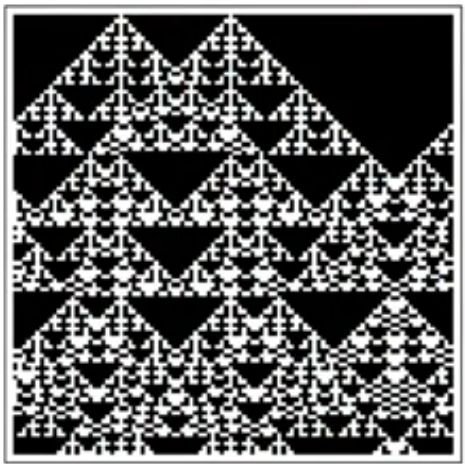
\includegraphics[width=\textwidth]{cellular-automaton-1}
		\end{subfigure}
		\hfill
		\begin{subfigure}[T]{0.3\textwidth}
			\caption{Another set of initial conditions}\label{fig:cellular-automaton-2}
			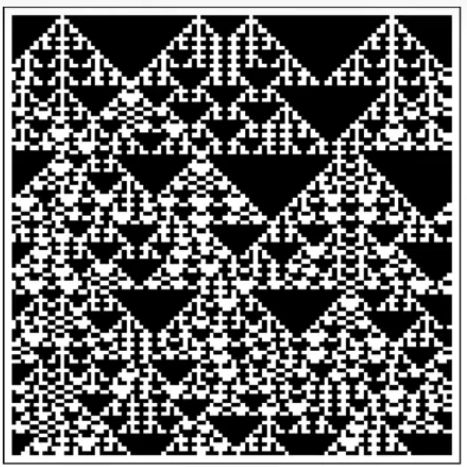
\includegraphics[width=\textwidth]{cellular-automaton-2}
		\end{subfigure}
		\hfill
		\begin{subfigure}[T]{0.3\textwidth}
			\caption{Random initial conditions}\label{fig:cellular-automaton-3}
			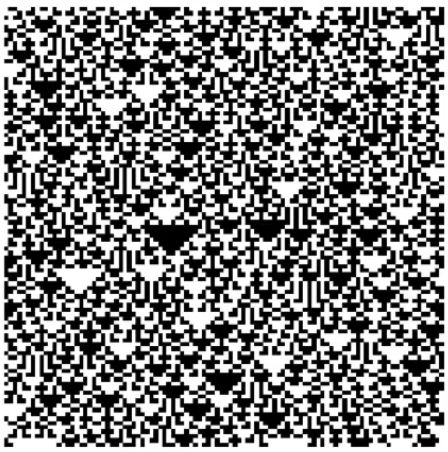
\includegraphics[width=\textwidth]{cellular-automaton-3}
		\end{subfigure}
	\end{center}
\end{figure}

How do you read Figure \ref{fig:cellular-automaton-1}?
Consider the very first line of pixels, at the top: you can see most of the pixels are black then there are two white pixels.
That's the state of the system at time $t$.
There is an evolution rule, a rule about how to go from that first line of pixels to that second line of pixels and from that second line of pixels to that third line of pixels and so on.
There is a rule that takes you from one line to the next and produces this kind of beautiful pattern that you see here.
So those two little points sort of explode and evolve over time spreading outwards and even interact with each other line sort of waves on a beach, that kind complicated patterns.

Figure \ref{fig:cellular-automaton-2} shows the same update rule with a different set of initial conditions. And now what you can see is that in fact whereas before be began with all black pixels except for two white ones now what I've done is add in another two white pixels. And again you see that same kind of triangular sort of expanding wave pattern. Another sort of a regular system evolves differently.

You see more complicated patterns the further down you go. Figure \ref{fig:cellular-automaton-3} shows one more example of again the same update rule
but now with random initial conditions.
So instead of sort of setting up almost everything with the black pixels
and somewhere white pixels now I've just randomly laid out black and white at that first line.
And you can see now as system evolves through time you kind of lose that very structure, the triangular propagating wave shape.
It's almost that you have just too many waves interacting with each other.
And you get kind of sort of big chunks of white and black triangles.
All of those pictures are generated by the same rule and that rule, in contrast to the Markov chain, is deterministic.
I can tell you with certainty what will happen to one pixel depending upon all the pixels just previous.
The rules themselves are incredibly simple. Figure \ref{fig:cellular-automaton-rule} zooms in on an example of the first three lines
of a cellular automaton. 

\begin{figure}[H]
	\begin{center}
		\caption[An example of the first three lines
		of a cellular automaton]{An example of the first three lines
			of a cellular automaton. The state of that pixel marked
			with the question mark depends solely upon the pixel just above it and just above it to the left and just above it to the right.}\label{fig:cellular-automaton-rule}
		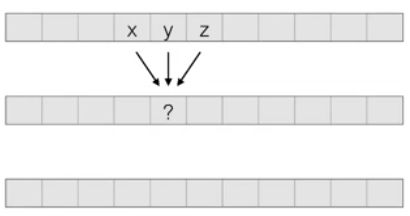
\includegraphics[width=0.6\textwidth]{cellular-automaton-rule}
	\end{center}
\end{figure}
Notice that this question mark pixel doesn't depend upon, let's say, something very far to the left or very far to the right and also, just to remind you of the kind of forgetful nature of the cellular automaton, it doesn't depend on the values of pixels
before the line just previous.
Of course I can use facts about the lines further up the screen to predict
what this question mark is going to do.
But once you tell me the value of pixel $x$, $y$, and $z$, you've determined, for all time, what will happen to the question mark pixel.
We call that function $f$; that function $f$ takes the three pixel values and tells you what will happen next.
And once I define the function $f$, I've defined the evolution rule of the cellular automaton, and all that remains for me is to lay down some initial conditions and use my computer to compute $f(x,y,z)$ for all the pixels at the next line.
You can think of this as a lookup table and because the pixels can either be black or white, let's say one or zero, now we have a lookup table.
I have two possible values for $x$, two possible values for $y$, and two possible values for $z$: $2^3=8$, eight possible values that could drive the value of
question mark pixel.
And my function $f$ has to tell you what happens for each of those possible eight combinations.
If you think about it if there are eight possible combinations and I have to specify one or zero for each of those eight, I now have $2^8=256$ different rules, two choices for each value of the triplet.
And so, for a cellular automaton defined by a neighbor rule like this one, there's only 256 possible rules that you can have.
There's only 256 distinct functions $f$.

Let's take look at the rule I've just showed you evolving. It's actually called rule 150.
\begin{figure}[H]
	\begin{center}
		\caption{Rule 150: $\big((x \xor y) \xor z\big)$}\label{fig:cellular-automaton-rule-2}
		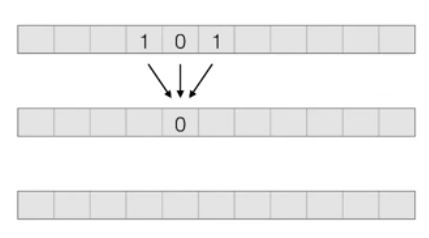
\includegraphics[width=0.6\textwidth]{cellular-automaton-rule-2}
	\end{center}
\end{figure}
There's a simple way to write that I can tell you, the lookup table, but it is also possible just to phrase it in terms of logical gates.
And you can phrase rule one-fifty as the value
of the x pixel XORed with the values of the y pixel and that value XORed with the value of the z pixel. 

Another way to talk about rule 150, another way verbally describe that function $f$ is not in terms of gates but just to say that the output is black when there's an odd number of black cells above.
In Figure \ref{fig:cellular-automaton-rule-3} we  watch rule 150 evolve over time.
\begin{figure}[H]
	\begin{center}
		\caption{Rule 150 evolving}\label{fig:cellular-automaton-rule-3}
		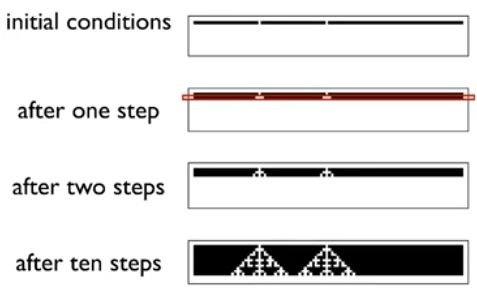
\includegraphics[width=0.6\textwidth]{cellular-automaton-rule-3}
	\end{center}
\end{figure}
We begin with these initial conditions and after one step what you can see is that the pixel just directly below that white pixel stays white because the value just above it is white, the value above it to the left is black, the value above it to the right is black, that's an even number of black pixels, so that pixel there stays white.
And now you can begin to see how that starts to spread out over time and the different ways in which these triangular patterns emerge.

That's rule 150. We can also consider a different rule. Figure \ref{fig:cellular-automaton-rule-4} depicts rule 105.
\begin{figure}[H]
	\begin{center}
		\caption{Three different rules}
		\begin{subfigure}[t]{0.3\textwidth}
			\caption{Rule 105}\label{fig:cellular-automaton-rule-4}
			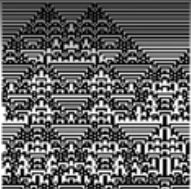
\includegraphics[width=\textwidth]{cellular-automaton-rule-4}
		\end{subfigure}
		\begin{subfigure}[t]{0.3\textwidth}
			\caption{Rule 90}\label{fig:cellular-automaton-rule-5}
			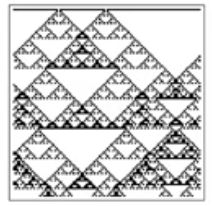
\includegraphics[width=\textwidth]{cellular-automaton-rule-5}
		\end{subfigure}
		\begin{subfigure}[t]{0.3\textwidth}
			\caption{Rule 110}\label{fig:cellular-automaton-rule-6}
			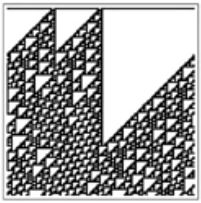
\includegraphics[width=\textwidth]{cellular-automaton-rule-6}
		\end{subfigure}
	\end{center}
\end{figure}
Of course because there's 256 possible $f$ rules
we're going to run out of them eventually.
There's a numbering system that people have invented and so usually when someone says rule 105 you can actually figure out exactly what that look up table will appear as.

Figure \ref{fig:cellular-automaton-rule-5} depicts rule 90.
You start to see some of these triangular patterns are quite familiar, the ways in which these triangles interact with each other.

Figure \ref{fig:cellular-automaton-rule-6} depicts a different one,
rule 110; you can see it's sort of asymmetrical.
So, even if I begin with the same initial conditions as I used for rule 150, instead of getting a triangle that sort of propagates out evenly in both directions
you kind of have asymmetry here, so in fact in Rule 110 a triangle propagates only in one direction and keeps a hard boundary on the other.

You can also see here which is kind of fun, it's quite clear now that rule 110 as the triangle propagates off the left edge we have it wrap around to the right edge.
So the neighbor of a pixel on the far right-hand side includes a pixel just up and to the right which wraps around to the far left.
In fact rule 110 is kind of a magical rule: it's what we call Turing universal.
Table \ref{table:rule-110} shows the lookup table. But the eight possible things that could happen give it a particular cell that you're wondering what its state is going to be.
\begin{table}[H]
	\caption[Lookup table for rule 110]{Lookup table for rule $110 = 64 + 32 + 8 + 4 + 2 = 2^6 + 2^5 + 2^3 + 2^2 +2^1$}\label{table:rule-110}
	\begin{tabular}{|l|c|c|c|c|c|c|c|c|}\hline
		Current pattern&111&110&101&100&011&010&001&000\\ \hline
		New state for centre cell&0&1&1&0&1&1&1&0\\ \hline
	\end{tabular}
\end{table}


Rule 110 is interesting because it turns out that it can compute any possible function. 
It's actually equivalent to a computer, to a piece of Python code.
So how does that work, how does that make sense?

One way to think of it is this. Imagine a piece of Python code that I want to execute I can of course just put it into a laptop and have it run. 
But if I'm really clever what I can do is I can take that Python code, turn it into a very long initial condition for rule 110, evolve rule 110 forward, wait for a certain amount of time and then read out at the bottom the output of that piece of Python code.
Of course the hard part is figuring out how to turn that Python code into a line of ones and zeros that form the input to rule 110.
It's not that easy.
But what Matthew Cook was able to do back in the early 2000s
was show that it is at least in principle possible to do that.\cite{cook2004universality}
In fact rule 110 given sufficiently rich initial conditions can perform an arbitrary computation.
It is in fact one way to implement a Turing machine if you know this language from computational theory.

So how did Matthew do it?
Well, it's kind of a fun way to play just to get a sense of how you might do it.
Figure \ref{fig:two:examples:rule110} presents two examples of how rule 110 behaves
given a particular set of initial conditions.
\begin{figure}[H]
	\caption{Rule 110 given a particular set of initial conditions}\label{fig:two:examples:rule110}
	\begin{subfigure}[t]{0.45\textwidth}
		\caption{Gliders--A4 and Ebar}\label{fig:cellular-automaton-rule-7}
		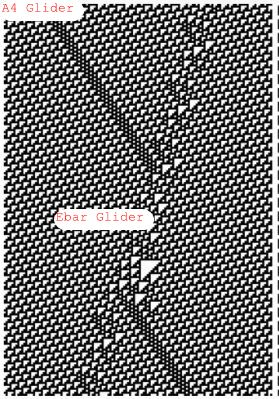
\includegraphics[width=\textwidth]{cellular-automaton-rule-7}
	\end{subfigure}
	\hfill
	\begin{subfigure}[t]{0.45\textwidth}
		\caption{Conversion of an EBar into a C2}\label{fig:cellular-automaton-rule-8}
		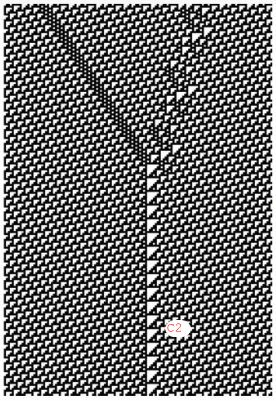
\includegraphics[width=\textwidth]{cellular-automaton-rule-8}
	\end{subfigure}
\end{figure}
What you can see here in Figure \ref{fig:cellular-automaton-rule-7} is all these different structures that appear you have what are called gliders.
So if you look at that sort of polka dot points or that polka dot stripe there Cook called this an A4 glider, and when an A4 glider meets what he calls an Ebar glider
which is a much more complicated pattern that propagates to the left the A4 glider and the Ebar glider depending upon exactly how they collide with each other
can either be absorbed, can change the state of the Ebar glider, and can lead to re-emission.

So Figure \ref{fig:cellular-automaton-rule-7} the A4 glider hits the Ebar glider,
kind of gets stored there for a while and gets spat out a little bit later
that A4 glider continues unimpeded but if it had hit the Ebar glider a little earlier
in its evolution in that case what we would have seen is that the Ebar and the A4 glider return into a stationary object, into a C2--Figure \ref{fig:cellular-automaton-rule-8}. And that C2 would stay stationary over time.

So what Cook was able to do is show that in fact all these little sort of discreet propagating structures that emerge naturally from rule 110 and there's no magic here in the sense that all of these patterns are produced solely by Rule 110.
Playing out the rule for each point what happened for each point is the state of each point is defined by the three units just above it.
It's just playing out that rule over and over and over again to produce these lines as they come down the page. What Matthew Cook was able to do was show this is essentially enough to produce what you might now think of as a set of logic gates or way a system could write things to a tape, read things back from the tape, do something to the value of that tape depending upon what it had read, and what else was happening elsewhere in the system.
So Rule 110 turns out to be not just a kind of playful way to make cool patterns,
but in fact something sufficient to describe arbitrarily complicated systems.

So this has been a little introduction to cellular automata. What I've tried to do is first of all of course tell you how it works, tell you what the rules are of this model and then try to give you a sense the great diversity of behaviors that we can see here.

We saw rule 150 producing these propagating triangles that overlap with each other.
We saw an example something like Rule 90, where it also produced that kind of triangle-like pattern but the rules of how those triangles interacted with each other
were slightly different, so visually it looked different.
Then of course something like Rule 110, which is even crazier. Here if you set things up correctly, not only do you get these propagating objects, these spreading waves or indeed even these packets moving around.
But in fact the logic of how those things interact with each other is sufficiently complicated that you can perform an arbitrary computation,
that you can actually for example run
a piece of Python code or C code or BASIC.
So cellular automata are actually much more
complicated than the Markov chains we considered
in part because whereas the Markov chains
the state at one point in time
depends solely upon N states just previous
here in fact if you look far enough back in time
the value of any particular point
is influenced by a huge number
of inputs from arbitrarily far away.
So the cellular automata even
though it has the same forgetfulness
as the Markov chain
and even though the rules
themselves are incredibly simple
the fact that the one-dimensional line that these rules operate on can be arbitrarily large means that we'll have, it will turn out, a new kind of problem for how to describe the system and in particular a new kind of problem when we come to renormalize the system because what we're going to do now is imagine taking one of these patterns produced by a cellular automata
Squinting at it in some way, producing a reduced description of that pattern and then trying to figure out the kinds of rules that that pattern could be described by.

\subsection{Israeli and Goldenfeld; projection and commuting diagrams }

In the first section you had a brief introduction to cellular automata. There's a lot more to say about it, but I at least got a chance to give you a taste for the different kinds of patterns that each of the different kinds of rules can produce and I even gave you a little bit of a sense of the magic of Rule 110 and 110 will come back a little bit later.

For now though what I'm going to talk about is how we can think about coarse-graining a cellular automaton.
When we go from the Markov chains of the previous section to the cellular automata  there's going to be one important change and that change is going to affect how we think about the renormalization process. If we go back to the finite state machines, to the Markov chain models, if you have a system that you observe every let's say one second time step, and then you decimate that system down,
you coarse-grain it and so you now observe the system every two time steps. 
The original model in order to get from $t+1$ to $t+2$, you needed to know your position among the $N$ states, you need to know which state you were in, and once you knew which state you're in you could figure out which state you were in at time $t+2$.

And similarly to go from time $t$ to $t+1$ you just had to know which state you were in at time $t$. It's a Markov chain and so what that means is that you have a finite and fixed number of states over time. When we came to coarse-grain that model 
we could still keep the same relationship. In order to know where you were at time $t+2$ all you had to do was know your position among all of the $N$ states of the
new updated model at time $t$. What that meant was that we stayed within the same model class when we dropped some of the time information. We could produce an $N$-state Markov chain that skipped every step if we had an $N$-state Markov chain at the finer-grained timescale. This changes completely when we come to the cellular automata.

So if we take that grid evolution algorithm that we introduced you to, what you saw was that to know what this the state of the system here is at time $t$ at time $t+1$,
you needed to know the state of these three grid squares just above it. And then to know the state of that point at time $t+2$ again, you only needed three pieces of information.
But imagine that we dropped, we coarse-grained, we decimated out the $t+1$ data.
What do you have to know about this or what do you have to know about the state of the system here to know the value of this point here? Ian Classie,???, one of the people I learned this technique from once said this is sort of like what a physicist would call a light cone because as you go further back in time in order to know the state of this point here you need to know the state of this point here, but in order to know the state at this point here you have to know the state of the system at 
these three points here.

\begin{figure}[H]
	\begin{center}
		\caption[Light Cone for a Cellular Automaton]{Light Cone for a Cellular Automaton. The cell in the third row depends on three cells in the middle, five in the top.}
		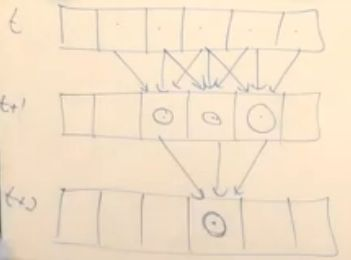
\includegraphics[width=0.8\textwidth]{cellular-automaton-light-cone}
	\end{center}
\end{figure}

And similarly to know the state of the system at this point here, you have to know the state of the system here and here as well.
And so as you go further and further back in time, as you drop this chunk of data here if you were to naively trying to do the same trick we did with the Markov chain
which is just come up with a model that work just as well to go from $t$ to $t+2$ you would find that instead of having a rule that looked like $f(x,y,z)$ your rule would now have to include five cells from the top row.
You'd have to in fact have five inputs to your function $f(a,b,c,d,e)$.

When you coarse-grain a cellular automaton only along the time dimension, you no longer stay within the same model class.
If you said, okay, produce a model that can get you from here to here that model would not fall in one of the 256 cellular automata that we introduced you to
in the first section of this module.
So, what do we do? Well, this is a trick that was introduced by a pair of scientists
Israeli and Goldenfeld\cite{israeli2004computational,israeli2006coarse}
and then I learned how to make it work in person from Ian Classie and Josh Grochow here at the Santa Fe institute.

But here's one story about how to solve this problem.
If you coarse-grained in time you don't stay within the same model class.
What Goldenfeld and Israeli did was ask you to think not about individual grid points
at this later time point, but pairs of grid points.
And then to look at the backwards light cone, the space of influence that this pair is subject to.
So, one step back, it's pretty easy: I just have to add one more point in the middle row.
\begin{figure}[H]
	\begin{center}
		\caption{Light Cone for pairs of cells}\label{fig:cellular-automaton-light-cone-pairs}
		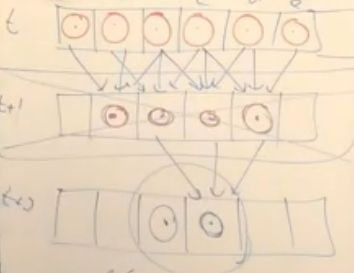
\includegraphics[width=0.8\textwidth]{cellular-automaton-light-cone-pairs}
	\end{center}
\end{figure}
So this is the set of grid points that I have to know in order to predict the state of this pair of grid points at time $t+2$ and then if I zoom one step further back
what you can see is that I just have to include an additional grid point here on the far left edge.
So these two grid points at time $t+2$ are influenced by all of these six grid points at time $t$. What Goldenfeld and Israeli then asked us to do was to consider the supercell in the third row as a unit, call this let's say $\hat{a}$ and these six cells in the top row, to group them into three supercell units $\hat{x}$, $\hat{y}$ and $\hat{z}$.
If you write it this way,
then the logic of
the fine-grained simulation
means that in fact the state
of the a $\hat{a}$ grid cell
is now equal to something, we'll call it $\hat{f}(\hat{x},\hat{y},\hat{z})$.
\begin{align*}
	\hat{a} = \hat{f}(\hat{x},\hat{y},\hat{z})
\end{align*}
So the state of this pair here, whether they're both on, this one's on and this one's off, this one's off and this one's on or they're both on, that state of that grid cell or that supercell here depends upon the state of these three supercells up here and this law here is given
in the same form as this law here with one change.
The original evolution law for the cellular automata takes binary variables, ones and zeros.
This evolution law here takes pairs of ones and zeroes instead of there being two possible states for each supercell there are four.
And while this one here outputs one or zero
this function here outputs 00, 01, 10 or 11.
So we're part of the way there to coarse-graining the cellular automata.
We're only part of the way, we have something that depends, we have a function that depends upon three arguments and spits out one.
That's an improvement over what we wanted to do before where we had a function that takes in five arguments.

The problem is is that these arguments are now no longer binary variables.
So, what do we do? Well, instead of coarse-graining just in time we can also
coarse-grain in space.
And what they introduced was a projection operator $P$, which takes the state of a supercell and maps it to a binary variable 0 or 1:
\begin{align*}
	P(\hat{x}) \in& \{0,1\}
\end{align*}
So explicitly there are four possible states the supercell can be in, and what the projection operator does is it maps some of them to 1 and it maps the rest of them to 0.
You can think of this projection operator here as something very similar to what we did in the introduction to this module altogether where I showed you how you could coarse-grain an image--in that case the image of Alice and Dinah, her kitten.
In this case here for example, we could imagine doing a spatial decimation where we take only the value of the first entry in the supercell.
That kind of spatial decimation would lead to a projection operator where two terms were mapped to 0 and the other two to 1.

So, now that we've introduced the projection operator, let's see where we are.
We began with the original evolution law of the fine-grained cellular automata $f(x, y, z)$.
We then realized that if we wanted to skip two time steps in the future we would have to have more arguments.
So we rewrote that as $\hat{f}(\hat{x},\hat{y},\hat{z})$.
This function takes the state of the system here and evolves it two steps forward.
Instead of writing each of these grid cells separately we write them as a combined variable $\hat{x}$, $\hat{y}$, and $\hat{z}$.
Now the relationship between this $f$ and this $\hat{f}$  is totally deterministic.
Once you tell me this I can work out this here.
The problem is is that this $\hat{f}$ is no longer in the same model class as $f$.
All I've told you is that when you coarse-grain in time, you get a different model.
But there's really no good way to relate these to say like oh this has become more or less complex, this has become more or less interesting,
this parameter has changed. We can't for example place these as dots in some phase space and show, how models move as you coarse-grain them in time.
But now we have the projection operator and so we can write something like this.
We can project down the input supercells.
We can coarse-grain the spatial state of the system, and then we can talk about
the function $g(P(\hat{x}), P(\hat{y}), P(\hat{z}))$ that evolves these coarse-grained variables forward in time.
So, we can think about these two different operations on a diagram that you can imagine as, well, it's sometimes called a commuting diagram.

\begin{figure}[H]
	\begin{center}
		\caption{Commutation diagram for \glsdesc{gls:CA}}
		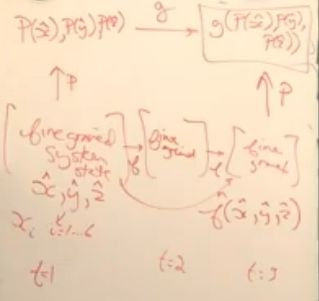
\includegraphics[width=0.8\textwidth]{commutation-2}
	\end{center}
\end{figure}
At the bottom, we have the fine-grained system state specified by three variables $\hat{x}$, $\hat{y}$, and $\hat{z}$.
And of course these variables here expand
if you wanted to into a list let's call them $\{x_i\: i \in [0,6]\}$ for that little patch of the cellular automaton.
So this is at time $t=1$, then we can get the fine-grained system at time $t=2$.
And then we can get the fine-grained system at $t=3$.
With the projection operator I can take this set of system states here
and map them to a set of projections $\hat{p}$ or $p(\hat{x})$,  $p(\hat{y})$ and  $p(\hat{z})$.
And then I can evolve that coarse-grained system forward using some function $g$.
Now what $g$ does is it takes in three binary variables and spits out a single binary variable so $g$ is somewhere in the model class of cellular automata, and out the other side I get a new set of variables or rather I get the evolved state of the system at the coarse-grained level.
From here to here we just require $f$ and $\hat{f}$.
And so going along the bottom we evolve the supercells.
Going up we project the initial configuration of the supercells.
Going right up here we evolve that projected configuration forward in time.
And so now we can compare what happens if you coarse-grain and evolve to what happens if you evolve and then coarse-grain.

So our goal now will be given a particular
cellular automata, $f$ at the fine-grained level,
can we find a projection operator $P$
and a coarse-grained evolution operator $g$
such that if you go along this path
it's equivalent to going along that path?
In other words, can we make this diagram
in the technical language, commute?
Notice that  this function here $g$ takes in three binary variables and spits out a single binary variable and so it is in fact
in this same Cellular Automaton model class
that is indeed one of the 256
of the cellular automata
that we can think about to begin with.
If we go with this projection
operator here
it may even be the case
that we can find a $P$ such that
the $g$ that makes this diagram commute is
is equal to the $f$. In other words
if we skip a step and blur
the spatial dimension in the right way
we may actually get back
the same evolution operator.
It's a little bit like saying
If you zoom out
and squint do you get back
the same process with which you began?

\subsection{Networks of Renormalization}

For Israeli and Goldenfeld it's all about taking one of two possible paths and getting to the same place.
\begin{enumerate}
	\item One path says I have a fine-grained description of the system
	I'm going to evolve it forward with my fine-grained rule and at the end I'm going to simplify the answer I'm gonna say look yes I mean I kept track of all these details but in fact you know what? I only need to know some of the output
	I only need to know some of the final stages of system 	So you can think of that as sort of walking along like this and then projecting up.
	\item Another way you can do it though 	right, is you can say look you give you this fine-grained description 	but I know I don't really care so much about this I'm going to project that down. 	Here's my fine-grain beginning initial condition 	I'm going to project that down to a simpler description and then I'm going to use a new rule that allows me to evolve
	that simplified description forward.
\end{enumerate}

So there are two paths and if you've done it right, they'll get you to the same place evolve the fine-grained system forward and project or project and evolve the coarse-grained description forward. A mathematician would say that these two operations \emph{commute}: you can do one or the other in either order,
and you'll get the same answer; A then B projecting then evolving is the same as B then A evolving and projecting.

So let's see how this plays out with a particular example. Again, I'll just take one from their paper, rule 105--Figure \ref{fig:cellular-automaton-rule-4a}.

\begin{figure}[H]
	\begin{center}
		\caption[Rule 105: $f_{105}(x_{n-1},x_n,x_{n+1})=\neg (x_{n-1} \xor x_n \xor x_{n+1})$]{Rule 105: $f_{105}(x_{n-1},x_n,x_{n+1})=\neg [x_{n-1} \xor x_n \xor x_{n+1}]$ Output is black when an even number of input cells is black.}\label{fig:cellular-automaton-rule-4a}
		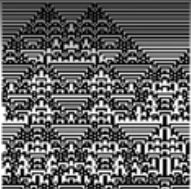
\includegraphics[width=0.6\textwidth]{cellular-automaton-rule-4}
	\end{center}
\end{figure}
 Rule 105 is quite similar to rule 150 which you've seen before: it takes the XOR of the three pixels above the pixel in question and then inverts them.
The only difference between rule 105 and 150 is that final inversion.
Another way to think of that is equivalently, the output is black when there's an even number of black cells above.

So now you know what we have to do. The first thing is we're going to consider not the final state of one pixel but the final state of two pixels. And we're going to ask what happens not when you take one time step but in fact when you take two time steps.
And that means that those two final pixels will depend on a group of six pixels
two time steps previously.
And now we'll consider those pairs of pixels to be the supercells.
So you have a big supercell here, which is two pixels, takes four possible states,
and you have three supercells up here: that's our $\hat{f}$.
What we have to do now is find a combination, a projection
$P$ that takes that supercell and summarizes it, simplifies it.

It maps each of those four possible states down to one of two possible states
We have a projection $P$ and we want to
find an evolution operator $g$
that allows us to evolve forward
those projected down superstates.
So the $P$ is what takes you from the
fine-grained descriptions up
to the coarse-grained description
and that $g$ is what's going to take you
between to coarse-grained descriptions
at different times.
So you can either go
f, f, f, f, f, p or
p, g, g

For every two times you iterate $f$ you're going only to iterate $g$ once and this simple example we'll just do the case where you skip one step and so you have supercells of size two.

Fortunately it turns out that it is possible to find a $P$ and $g$ that enable that diagram to commute and here it is in the case of Rule 105

\begin{figure}[H]
	\begin{center}
		\caption[Rule 105 can be made to commute]{If we take this as our projection function, rule 105 can be made to commute if we use rule 150.}\label{fig:rule105-P}
		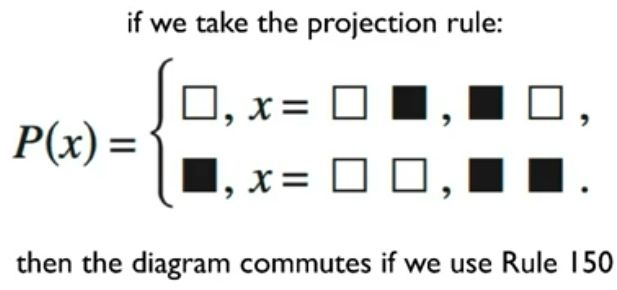
\includegraphics[width=0.6\textwidth]{rule105-P}
	\end{center}
\end{figure}
In this case the projection rule says if the supercell has one cell that's black and one cell that's white, make that all white; if both cells are white or both cells or black then make it black.
It's sort of like an extra rule itself in fact.
Actually, it looks a little bit like an edge detector: if there's a difference within the supercell mark it one way; if there's no difference in the supercells that are homogeneous mark it the other way.

If you use that projection operator then it turns out in fact that your $g$,
which is now of course taking binary values, take a binary value because you projected the four possible states supercell down to a cell.
It only has one of two possible states,
and that's what $g$ operates on,
that $g$ evolution operator actually turns out to be rule 150.
So what we've shown
is that it's possible to find a non-trivial coarse-graining and an evolution operator that's still within the space of
cellular automata  that enables that diagram to commute.
And so now just as we were able to talk about different kinds of
Markov chains coarse-graining into each other
we're now able to talk about how
rules coarse-grain into each other.
And in fact for a non-trivial projection operator Rule 105 coarse-grains into rule 150.
Here's what it looks like.
\begin{figure}[H]
	\caption[Rule 105 coarse-grains into rule 150]{Rule 105 coarse-grains into rule 150 by a non-trivial projection operator (based on a figure in \cite{israeli2004computational})}\label{fig:105:coarse:grained}
	\begin{subfigure}[t]{0.45\textwidth}
		\caption{Rule 105: Fine-grained level}\label{fig:fine:grain}
		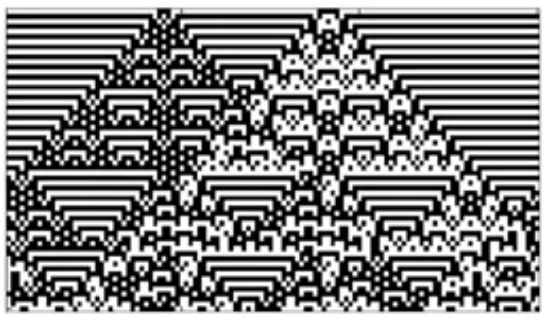
\includegraphics[width=\textwidth]{fine-grain-ca}
	\end{subfigure}
	\hfill
	\begin{subfigure}[t]{0.45\textwidth}
		\caption{Rule 150: coarse-grained level}
		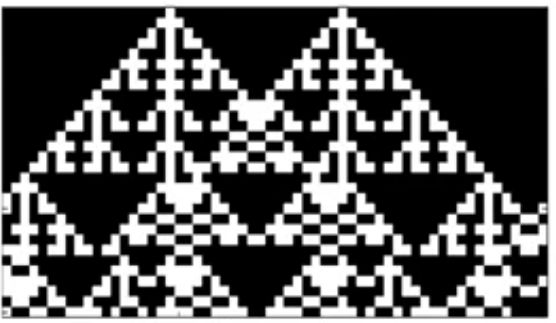
\includegraphics[width=\textwidth]{coarse-grain-ca}
	\end{subfigure}
\end{figure}

In Figure \ref{fig:fine:grain} you can see that we have the smaller pixels and those smaller pixels are both small in the x direction along this axis here and smaller in the time direction then in the coarse-grained case.
The coarse-grained case of course lumps pairs of states into one and then in fact the jumps are now larger there are two time steps instead of one.
And by looking at the the comparison between these two
you can sort of see what's going on.

First of all, the coarse-grained description is capturing something interesting about the fine-grained description.
We still have this idea that these triangles, these little perturbations that we begin with that lead to these expanding waves,  we still get that kind of wave like texture.
These sort of propagating spaces that have kind of internal structure
But you can also see that we are missing things too, right?
So if you look at those two triangles at the fine-grained level
one of them is sort of darker than the other
But in fact when we coarse-grain the differences
between those two triangles goes away.
So somehow rule 150
when we evolve it forward is
operating our coarse-grained descriptions.
That's thrown out some interesting features of Rule 105
another obvious feature here that
distinguishes rule 105 from rule 150
is that we lose that kind of zebra
stripe pattern
and that's of course because if
A pair of squares is both white
or both black
the projection operator maps them both
into a square that's both black.
So we've lost some of the structure
both in the sort of places
where those opening
Propagating triangle waves have
sort of reached it
and also within the triangles themselves
This gives you a little bit of a better sense

As we'll see it's not always the case that the picture that you get when you coarse-grain looks similar in some important respects to the fine-grained descriptions.
Figure \ref{fig:105:coarse:grained} is a particularly elegant example
of how we we're able to capture something about the rule
But of course not everything
we can't really capture everything of course
because that projection operator
is a lossy compression,
it throws out information.
And for rule 105 it really matters
whether everything is white or everything is black
But in fact the rule 150 when
we do the projection
it masks both of those cases to the same state.

\begin{figure}[H]
	\begin{center}
		\caption[Mapping one rule set to another by projection]{Mapping one rule set to another by projection after \cite{israeli2006coarse}}\label{fig:ig-relationships}
		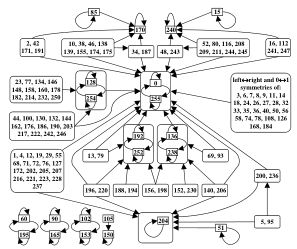
\includegraphics[width=0.8\textwidth]{ig-relationships}
	\end{center}
\end{figure}
Israeli and Goldenfeld looked at all 256 rules, and  tried to figure out how or the extent to which one rule could coarse-grain into another.
So these arrows in Figure \ref{fig:ig-relationships} show you how it's possible
to find whether or not it's possible to find a projection operator and an evolution operator that allows one rule set to map to another upon that coarse-graining.
They consider not only supercells of size 2 but also size 3 and size 4 and and computation of this starts getting really hard because there's so many different kinds of projection operators you can use and there's so many different possible evolutions that you can pick that you start to run out of time it gets exponentially hard to find a good projection operator, that gets exponentially hard to search the space. There's only a partial map, but what you can see here is for example
in the bottom the result that we just talked through a little bit laboriously which is the fact that it's possible to find a projection operator that takes you from state 105 or from evolution rule 105 to evolution rule 150.

By the way one of the things you can notice from this graph is that it's clear that
Israeli and Goldenfeld haven't actually found every possible coarse-graining relationship.
And that's because there should be a feature of this network that doesn't actually happen.
And that's that if A coarse-grains into B If A renormalizes into B, if it's possible to find a projection and evolution operator to take A and B and B renormalizes into C
it's possible to find a projection that takes B into C then it should also be possible to renormalize A into C of course now you're going to be coarse-graining twice and it's harder of course for Israeli and Goldenfeld to find those
but if you look at this chart what you should see is for example the fact that not only does rule 23 coarse-grain to rule 128 and not only does rule 128 coarse-grain to rule 0 but it also should be the case that it's possible for rule 23
to coarse-grain all the way down to rule 0 just by doing two projections and zooming out even further.
That said Israeli and Goldenfeld did a pretty good job looking at an enormous number of possible relationships between all of these possible rulesets. I find these diagrams quite compelling. They tell you something really complicated, really interesting about how deterministic rules and deterministic projections map into each other other.

One of the things that you'll see from that network is that not only does rule 105
coarse-grains to rule 150 but in fact rule 150 coarse-grains into itself:
it is a fixed point of renormalization group. With that projection operator you actually take rule 150 into a zoomed-out version of itself.
You sort of skip a step, you project down the supercells and you recover the same rules.
Now it's important to notice there's a subtlety here, right.
It doesn't mean that the image itself is self-similar doesn't necessarily mean the rule 150 is kind of fractal in some interesting way.
Because the coarse-graining may not be the kind of coarse-graining that just simply zooms out.
Consider for example the projection we had going from rule 105 to 150.
Now wasn't a simple decimation in the way that we did on the Alice picture for example at the beginning of this renormalization module.
In that case, right, we're renormalizing Alice.
We took her picture, we looked at little packages of cells, and we just take one of the values to define the value of that that larger grid cell that's supercell in the Alice case.
But if you remember the rule 105 to rule 150 projection that worked and that case
was actually an edge detector.
If the cell was all white or all black it got mapped to something that was all black.
So it doesn't necessarily mean that if you kind of fuzz rule 150 it still looks like rule 150.
It really depends upon the details of that projection operator.
That said in fact you might think of it another way.
Rule 150 is a fixed point of renormalization group with potentially a much more interesting projection than a simple decimation.

\begin{figure}[H]
	\begin{center}
		\caption{Coarse-graining Rule 110}\label{fig:cellular-automaton-rule-6a}
		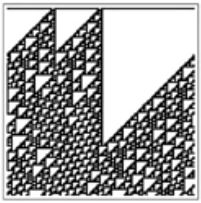
\includegraphics[width=0.6\textwidth]{cellular-automaton-rule-6}
	\end{center}
\end{figure}

Recall that Rule 110 is Turing complete: given a suitably specified initial condition, we can evolve the rule to perform an arbitrary computation. Can I coarse-grain the output, using Israeli and Goldenfeld's methods, to speed up the computation? Israeli and Goldenfeld were able to find projections, but they discarded almost all of the initial information. They exploited ''Garden of Eden States'', which can serve as an initial pattern, but can never be produced by evolution Rule 110 has Garden of Eden States: if $P$. projects Garden of Eden states to black, and all others to white, it doesn't do anything useful. Rule 110 coase grains to Rule 0.


What is we ask for an evolution rules that works with a specified projection, such as the Alice projection of Figure \ref{fig:rule90-alice}? it turns out that we cannot. Consider the inset: why did this bit switch on? It makes sense in the full view to the left, but not the decimated one on the right. What makes one time steo different from another?

\begin{figure}[H]
	\begin{center}
		\caption[Rule 90 with Alice coarse-graining]{Rule 90 with Alice coarse-graining. On the right we have thrown away all but one pixel from each decimation area.}\label{fig:rule90-alice}
		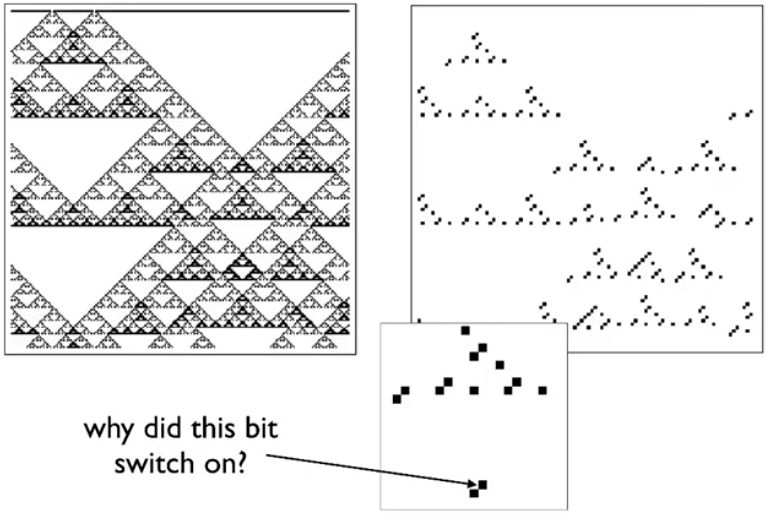
\includegraphics[width=0.8\textwidth]{rule90-alice}
	\end{center}
\end{figure}

A coarse-grained cellular automaton may no longer have a local update rule: distant points may be needed eo explain why a point flicked. Rule 90 is non-renormalizable under the Alice decimation: we need another model.

Just because you simplify the description, it doesn't mean the model simplifies.

We'll return to how renormalization can induce long-range couplings and interactions in the next unit, on the Ising Model. If a theory extends in time as well as space, we can think about long-range couplings as a new form of memory: if I'm directly coupled to distant times, I have a new form of memory. For an unusual perspective on the relationship between renormalization and memory, see \cite{dedeo2018origin}

\section{Ising Model}

\subsection{Fixing a projection: From \glsdescplural{gls:CA} to Ising}
We now have two examples of how renormalization works, of the effects of coarse-graining in time:
\begin{itemize}
	\item Markov Chain--everything flows to lower dimensional subspace; first example of fixed point.
	\item \gls{gls:CA} --in order to stay within same model class, forced to coarse-grain in space also. Can coarse-grain universal rule 110, but projection is practically trivial, as the projection exploits Garden of Eden states. What if we specified the projection ahead of time? E.g use majority voting. Sometimes we get two different trajectories in the coarse grained states.Then we get non locality. 
\end{itemize}

When we coarse-grain a new model, the Ising model, we also lose locality! Arbitrarily long interactions arise. 
\subsection{Introduction to the Ising Model}

The Ising model is one of the classic toy models in the physical sciences for understanding collective behaviour. The Ising model was invented to describe the behaviour of atoms  on a lattice. We will do a 2 dimensional lattice. 

\begin{figure}[H]
	\begin{center}
		\caption[Ising Model: atoms arranged on a 2 dimensional lattice]{Ising Model: atoms arranged on a 2 dimensional lattice. The spin is shown for one atom only. In reality the ''lattice'' could be a network}
		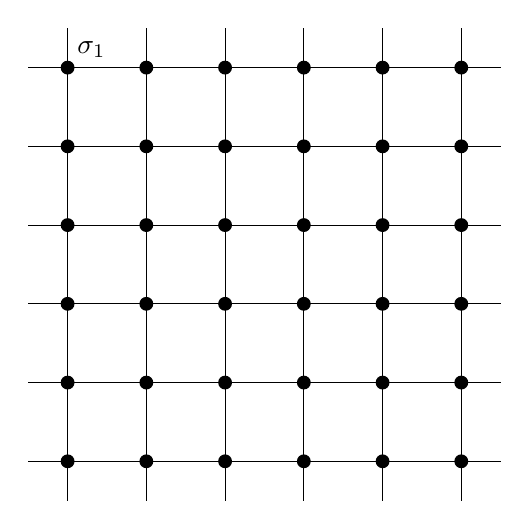
\begin{tikzpicture}
			\draw(-0.5,-0.5) grid (5.5,5.5);
			\draw[line width=5pt, line cap=round, dash pattern=on 0pt off 1cm](0,0) grid (5,5);
			\draw (0,5) node[anchor=south west] {$\sigma_1$};
		\end{tikzpicture}
	\end{center}
\end{figure}

Each atom has spin $\sigma=\pm 1$; this is a simplification of the actual state of an atom. In the Ising model, if two atoms are connected by an edge--graph theoretically they are near each other-- they will ''want'' to be in the same state. There is no causality propagating through the system; there is a general propensity for neighbours to find themselves in the same state. The Ising model is just a mathematical specification for things that are near each other wanting to be like each other.

We talk about a probability distribution over all states, $P(\{\sigma_i\})$ The probability of a configuration is given by:

\begin{align*}
	P(\{\sigma_i\}) =& \frac{e^{\beta \sum_{i,j} J_{i,j} \sigma_i \sigma_j}}{Z(\beta)}\text{, where} \numberthis \label{eq:coarse_ising:P} \\
	J_{i,j} =& 1,\text{if $i$ and $j$ are neighbours (connection or adjacency matrix)}\\
	=& 0 \text{ otherwise.}\\
	\beta =& \frac{1}{T} \text{, where $T$ represents the ''temperature''}\\
	Z(\beta) =& \text{ the partition function (normalization constant).}
\end{align*}
 
If two neighbours are both positive or both negative, $J_{i,j} \sigma_i \sigma_j$ will make a positive contribution to the probability: we add the adjacent pairs that are in the same state, and subtract those that are in different states. As $\beta$ increases, the benefit of all being in the same state gets larger.

The Ising model can also be used to model alignment of opinions, in which case the adjacency corresponds to communication.

How are we going to coarse-grain the Ising model? We will start with a very simple coarse-graining, where we take one node, A say, as shown in Figure \ref{fig:ising-coarse1}, and construct the joint probability distribution for all the other nodes. We will take the probability distribution for all other nodes, then sum over the possible values for $\sigma_A$.

\begin{figure}[H]
	\begin{center}
		\caption{Simple coarse-graining, based on $\sigma_A$}\label{fig:ising-coarse1}
		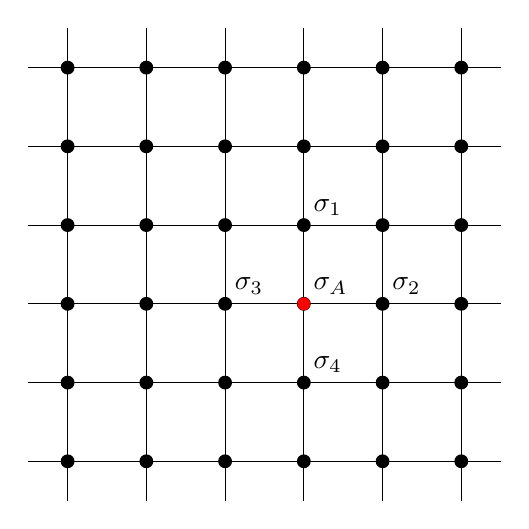
\begin{tikzpicture}
			\draw(-0.5,-0.5) grid (5.5,5.5);
			\draw[line width=5pt, line cap=round, dash pattern=on 0pt off 1cm](0,0) grid (5,5);
			\draw (3,2) node[anchor=south west] {$\sigma_A$};
			\draw (3,3) node[anchor=south west] {$\sigma_1$};
			\draw (4,2) node[anchor=south west] {$\sigma_2$};
			\draw (2,2) node[anchor=south west] {$\sigma_3$};
			\draw (3,1) node[anchor=south west] {$\sigma_4$};
			\draw[red,fill=red] (3,2) circle (.5ex);
		\end{tikzpicture}
	\end{center}
\end{figure}

When we do this, most things are not going to change: terms that don't involve $\sigma_A$ won't be affected. We therefore focus on the terms with $\sigma_A$. We will:
\begin{enumerate}
	\item pull out the term in the sum with $\sigma_A$;
	\item average out (''trace out'') $\sigma_A$.
\end{enumerate}

Then (\ref{eq:coarse_ising:P}) becomes:
\begin{align*}
	P(\{\sigma_i\}) =& \frac{\big[e^{\beta(\sigma_1\sigma_A + \sigma_2\sigma_A + \sigma_2\sigma_A + \sigma_4\sigma_A)}\big]B}{Z(\beta)} \text{ for fixed $\sigma_A$, where}\\
	B =& e^{\sum e^{\beta \sum_{i,j \ne A} J_{i,j} \sigma_i \sigma_j}}\\
	\sum_{\sigma_A=\pm 1} P(\{\sigma_i\}) =& \big[e^{\beta(\sigma_1+\sigma_2+\sigma_3+\sigma_4)} + e^{-\beta(\sigma_1+\sigma_2+\sigma_3+\sigma_4)}\big]  \frac{B}{Z(\beta)}\\
	=& 2 \cosh({\beta(\sigma_1+\sigma_2+\sigma_3+\sigma_4)})   \frac{B}{Z(\beta)}\\
	=& e^{\log{\cosh({\beta(\sigma_1+\sigma_2+\sigma_3+\sigma_4)})}} \frac{B}{Z^\prime(\beta)} \text{, absorbing $2$ in $Z^{\prime}$.} \numberthis \label{eq:coarse_ising:P2}
\end{align*}

Comparing (\ref{eq:coarse_ising:P}) and (\ref{eq:coarse_ising:P2}), we see that coarse-graining has complicated the equation. However, Table \ref{table:ising-cosh} suggests a way forward.

\begin{table}[H]
	\begin{center}
		\caption[Analyzing the $\ln \cosh$ term]{Analyzing the $\ln \cosh$ term in $ e^{\log{\cosh({\beta(\sigma_1+\sigma_2+\sigma_3+\sigma_4)})}} \frac{B}{Z^\prime(\beta)}$}\label{table:ising-cosh}
		\begin{tabular}{|l|l|l|}\hline
			\#&Neighbour configurations&Value of $\ln \cosh$ terms\\\hline
			1&All positive or all negative&$\ln \cosh 4\beta$\\\hline
			2&One positive, three negative (or vice versa)&$\ln \cosh 2\beta$\\\hline
			3&Two positive, two negative&$\ln \cosh 0 = \ln 1 = 0$\\\hline
		\end{tabular}
	\end{center}
\end{table}

\begin{thm}[Renormalizing Ising Model]
	\begin{align*}
		\sum_{\sigma_A=\pm 1} P(\{\sigma_i\}) \propto&e^{S_2 (\sigma_1\sigma_2 + \sigma_1\sigma_3+ \sigma_1\sigma_4 + \sigma_2 \sigma_3 + \sigma_2 \sigma_4 +\sigma_3 \sigma_4) + S_4 \sigma_1 \sigma_2 \sigma_3 \sigma_4} \numberthis \label{eq:coupled:sigmas}\\
		 \text{where}\\
		S_2 =& \frac{1}{8} \ln{\cosh{4\beta}} \tag*{pairwise interactions}\\
		S_4 =& \frac{1}{8} \ln{\cosh{4\beta}} - \frac{1}{2} \ln{\cosh{2\beta}} \tag*{quartet interaction.}
	\end{align*}
		Subject to a constant factor, which can be absorbed in the partition function.
\end{thm}

\begin{proof}
	We represent each of the three cases in Table \ref{table:ising-cosh} by an exemplar.
	\begin{table}[H]
		\caption[Exemplars for Table \ref{table:ising-cosh}]{Exemplars for Table \ref{table:ising-cosh}, where $\Sigma=\sigma_1\sigma_2 + \sigma_1\sigma_3+ \sigma_1\sigma_4 + \sigma_2 \sigma_3 + \sigma_2 \sigma_4 +\sigma_3 \sigma_4$}
		\begin{tabular}{|c|c|c|c|c|c|c|c|c|c|}\hline
			Case&Exemplar&$\sigma_1\sigma_2$&$\sigma_1\sigma_3$&$\sigma_1\sigma_4$&$\sigma_2\sigma_3$&$\sigma_2\sigma_4$&$\sigma_3\sigma_4$&$\Sigma$&$\sigma_1\sigma_2\sigma_3\sigma_4$\\ \hline
			1&$\sigma_i>0\;\forall i$&$+1$&$+1$&$+1$&$+1$&$+1$&$+1$&$+6$&$+1$\\ \hline
			2&$\sigma_4<0\;\forall i\ne 4$&$+1$&$+1$&$-1$&$+1$&$-1$&$-1$&$0$&$-1$\\ \hline
			3&$\sigma_{1,2}>0\land\sigma_{3,4}<0$&$+1$&$-1$&$-1$&$-1$&$-1$&$+1$&$-2$&$+1$\\ \hline
		\end{tabular}
	\end{table}
	Then we try to find $S_1$, $S_2$ and $C$ such that:
	\begin{align*}
		\sum_{\sigma_A=\pm 1} P(\{\sigma_i\}) =&e^{S_2 (\sigma_1\sigma_2 + \sigma_1\sigma_3+ \sigma_1\sigma_4 + \sigma_2 \sigma_3 + \sigma_2 \sigma_4 +\sigma_3 \sigma_4) + S_4 \sigma_1 \sigma_2 \sigma_3 \sigma_4}+C \text{. We need}\\
		6 S_2 + S_4 =& \ln \cosh 4\beta + C \numberthis \label{eq:S2:4:a}\\ 
		-S_4 =& \ln \cosh 2\beta+C\numberthis \label{eq:S2:4:b}\\ 
		-2S_2+S_4 =& C \numberthis \label{eq:S2:4:c}
	\end{align*}
	From \eqref{eq:S2:4:a} and \eqref{eq:S2:4:c}
	\begin{align*}
		8S_2 =& \ln \cosh 4\beta\\
		S_2 =& \frac{1}{8} \ln \cosh 4\beta \text{,  \eqref{eq:S2:4:b} and \eqref{eq:S2:4:c} give:}\\
		-2S_2 =& \ln \cosh 2\beta + 2C\\
		C =& -S_2 - \frac{1}{2} \ln \cosh 2\beta \text{, then \eqref{eq:S2:4:b} becomes}\\
		S_4 =& - \ln \cosh 2\beta - C\\
		=& - \ln \cosh 2\beta + S_2 + \frac{1}{2} \ln \cosh 2\beta\\
		=& \frac{1}{8} \ln \cosh 4\beta  - \frac{1}{2} \ln \cosh 2\beta
	\end{align*}

\end{proof}

Notice that (\ref{eq:coupled:sigmas}) couples $\sigma_1$, $\sigma_2$, $\sigma_3$, \emph{and} $\sigma_4$! This includes longer range couplings, such as $\sigma_2, \sigma_3$, plus the quartet! [There is also a constant factor that can be absorbed.] We have taken things that weren't coupled, and coupled them. Previously $\sigma_1$ and $\sigma_2$ didn't care about each other, but now we have removed the mediating variable $\sigma_A$, so now they do care in the renormalized case.

The lattice has also become a hypergraph.

Renormalizing has two effects: it changes the structure of the adjacency matrix, and it also introduces new types of interaction.
\begin{align*}
	P^\prime(\{\sigma_i\}) =& \frac{e^{\beta\big(J^\prime_{ij}\sigma_i\sigma_j+K_{ijkl}\sigma_i\sigma_j\sigma_k\sigma_l\big)}}{Z^\prime(\beta)}
\end{align*}
We have gone outside the model!

\subsection{Coarse-graining the Lattice}

\begin{figure}[H]
	\begin{center}
		\caption[Coarse-graining the Lattice]{Coarse-graining the Lattice. The decimation will throw out the $\sigma_A$ and retain the $\sigma_i$.}\label{fig:ising-decimation}
		\begin{subfigure}[t]{0.45\textwidth}
			\begin{center}
				\caption{The $S2$ couplings, \eqref{eq:coupled:sigmas}, are shown in blue. Note that each blue segment actually contributes $2S2$, as there are contributions from the two $S_A$s on each side.}\label{fig:ising-decimation:S2}
			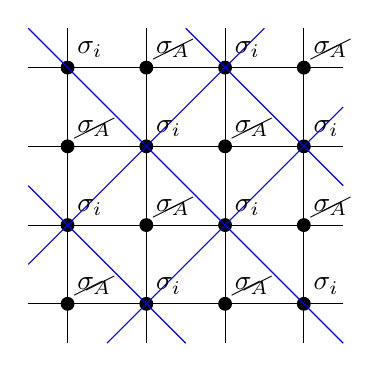
\begin{tikzpicture}
				\draw(-0.5,-0.5) grid (3.5,3.5);
				\draw[line width=5pt, line cap=round, dash pattern=on 0pt off 1cm](0,0) grid (3,3);
				\draw[blue] (3.5,2.5) -- (0.5,-0.5);
				\draw[blue] (2.5,3.5) -- (-0.5,0.5);
				\draw[blue] (-0.5,3.5) -- (3.5,-0.5);
				\draw[blue] (1.5,3.5) -- (3.5,1.5);
				\draw[blue] (1.5,-0.5) -- (-0.5,1.5);
				\draw (1,2) node[anchor=south west] {$\sigma_i$};
				\draw (2,2) node[anchor=south west] {$\cancel{\sigma_A}$};
				\draw (3,2) node[anchor=south west] {$\sigma_i$};
				\draw (0,2) node[anchor=south west] {$\cancel{\sigma_A}$};
				\draw (1,3) node[anchor=south west] {$\cancel{\sigma_A}$};
				\draw (2,3) node[anchor=south west] {$\sigma_i$};
				\draw (3,3) node[anchor=south west] {$\cancel{\sigma_A}$};
				\draw (0,3) node[anchor=south west] {$\sigma_i$};
				\draw (1,1) node[anchor=south west] {$\cancel{\sigma_A}$};
				\draw (2,1) node[anchor=south west] {$\sigma_i$};
				\draw (3,1) node[anchor=south west] {$\cancel{\sigma_A}$};
				\draw (0,1) node[anchor=south west] {$\sigma_i$};
				\draw (1,0) node[anchor=south west] {$\sigma_i$};
				\draw (2,0) node[anchor=south west] {$\cancel{\sigma_A}$};
				\draw (3,0) node[anchor=south west] {$\sigma_i$};
				\draw (0,0) node[anchor=south west] {$\cancel{\sigma_A}$};
			\end{tikzpicture}
			\end{center}
		\end{subfigure}
			\hfill
			\begin{subfigure}[t]{0.49\textwidth}
				\begin{center}
					\caption{One of the $S4$ couplings, \eqref{eq:coupled:sigmas}, is shown in green, and a long distance $S2$ coupling in blue.}\label{fig:ising-decimation:S4}
				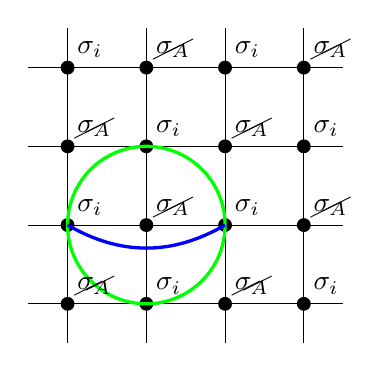
\begin{tikzpicture}
					\draw(-0.5,-0.5) grid (3.5,3.5);
					\draw[line width=5pt, line cap=round, dash pattern=on 0pt off 1cm](0,0) grid (3,3);
					\draw[green,very thick] (1,1) circle (1);
					\draw (1,2) node[anchor=south west] {$\sigma_i$};
					\draw (2,2) node[anchor=south west] {$\cancel{\sigma_A}$};
					\draw (3,2) node[anchor=south west] {$\sigma_i$};
					\draw (0,2) node[anchor=south west] {$\cancel{\sigma_A}$};
					\draw (1,3) node[anchor=south west] {$\cancel{\sigma_A}$};
					\draw (2,3) node[anchor=south west] {$\sigma_i$};
					\draw (3,3) node[anchor=south west] {$\cancel{\sigma_A}$};
					\draw (0,3) node[anchor=south west] {$\sigma_i$};
					\draw (1,1) node[anchor=south west] {$\cancel{\sigma_A}$};
					\draw (2,1) node[anchor=south west] {$\sigma_i$};
					\draw (3,1) node[anchor=south west] {$\cancel{\sigma_A}$};
					\draw (0,1) node[anchor=south west] {$\sigma_i$};
					\draw (1,0) node[anchor=south west] {$\sigma_i$};
					\draw (2,0) node[anchor=south west] {$\cancel{\sigma_A}$};
					\draw (3,0) node[anchor=south west] {$\sigma_i$};
					\draw (0,0) node[anchor=south west] {$\cancel{\sigma_A}$};
					\path [bend right, blue, very thick] (0,1) edge (2,1);
				\end{tikzpicture}
				\end{center}
			\end{subfigure}

	\end{center}
\end{figure}

Figure \ref{fig:ising-decimation} shows a decimation of the entire lattice. It exhibits 3 types of coupling:

\begin{enumerate}
	\item the survivors form a new lattice rotated $45^\circ$, with coupling $2S_2=\frac{1}{4} \log{\cosh{4 \beta}}$\label{item:coupling1}--Figures \ref{fig:ising-decimation:S2} and \ref{fig:ising-decimation-aoki}.
	\item long range couplings, over a deleted $S_A$,  $S_2=\frac{1}{8} \log{\cosh{4 \beta}}$\label{item:coupling2}--Figure \ref{fig:ising-decimation:S4};
	\item quartet couplings $S4=\frac{1}{2} \log{\cosh{2\beta}}$\label{item:coupling3}--Figure \ref{fig:ising-decimation:S4}.
\end{enumerate}

\begin{figure}[H]
	\caption{Coarse-graining the Lattice(after \cite{aoki2014domain})}\label{fig:ising-decimation-aoki}
	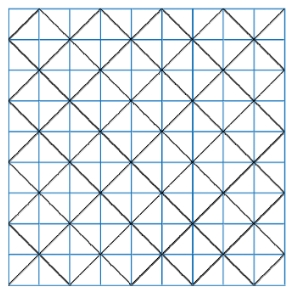
\includegraphics[width=0.9\textwidth]{isinng-decimation}
\end{figure}


If we can ignore couplings \ref{item:coupling2} \& \ref{item:coupling3}, we have transformed original lattice with coupling $\beta$ into one with coupling \ref{item:coupling1}: $\frac{1}{4} \log{\cosh{4\beta}}$.

\begin{thm}[Monotonicity of Ising Decimation]
	$\beta > 0 \implies \frac{1}{4} \log{\cosh{4\beta}} < \beta$
\end{thm}

\begin{proof}
	We will rearrange the demonstrandum to get it into a simpler form.
	\begin{align*}
		 \frac{1}{4} \log{\cosh{4\beta}} <& \beta\\
		 \iff&\\
		 \log{\cosh{4\beta}} <& 4\beta\\
		 \iff&\text{ transforming $\beta\rightarrow\frac{\beta}{4}$}\\
		 \log{\cosh{\beta}} <& \beta\\
		 \iff&\text{$exp$ is monotonic}\\
		 \cosh{\beta} <& e^{\beta}\\
		 \iff& \text{ Definition of $\cosh$}\\
		 \frac{e^{\beta}+e^{-\beta}}{2}<&e^{\beta}\\
		 \iff&\\
		 \cancel{e^{\beta}}+e^{-\beta}<\cancel{2}&e^{\beta}\\
		 \impliedby&\\
		 \beta<&0 \text{, by hypothesis}
	\end{align*}

\end{proof}

Since coupling decreases as we zoom out, we are less and less likely to see big domains that are aligned the same way. NB: this is not the same as previous Markov and Cellular automata, where we performed exact renormalization; this is approximate.

This is a bad approximation, as it ignores important interactions. We can do better by ignoring coupling \ref{item:coupling3} (quartet) and lumping \ref{item:coupling1} and \ref{item:coupling2}, new coupling $\frac{3}{8} \log{e^{2\beta} }$. This is a heuristic, but, apparently, doesn't work too badly.


See also \cite[Chapter 14]{kadanoff2000statistical}


\subsection{Finding Fixed Points}

How does model flow as we continue to coarse-grain? This replaces the lattice with another:  $\beta\rightarrow\frac{3}{8} \log{\cosh{4\beta} }$. Figure \ref{fig:beta} shows the behaviour of the function $\frac{3}{8} \log{\cosh{4\beta} }$ shows the evolution of the solution of  $\beta=\frac{3}{8} \log{\cosh{4\beta} }$. For small $\beta$ the solution evolves to $\beta=0$, and for large $\beta$ to $\beta=\infty$ ($T=0$).


\begin{figure}[H]
	\caption{The effect of repeated decimation: solving $\beta=\frac{3}{8} \log{\cosh{4\beta} }$}\label{fig:beta}
	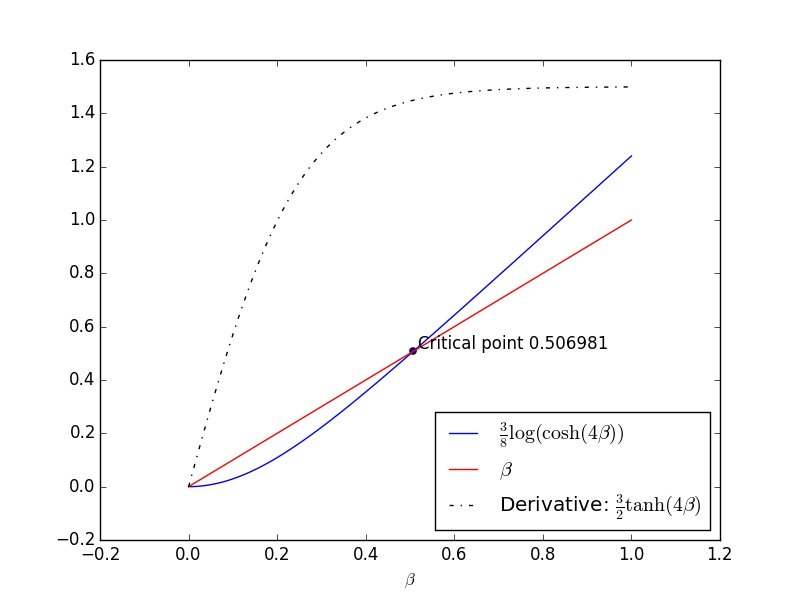
\includegraphics[width=0.9\textwidth]{beta}
\end{figure}

Figure \ref{fig:beta} shows that the mapping $\beta\rightarrow\frac{3}{8} \log{\cosh{4\beta} }$ has three fixed points. There are three scenarios for repeated decimation.
\begin{enumerate}
	\item $\beta=0$: as we zoom out, spins become random over a large area, and there is no long range correlation.
	\item  $\beta=\infty$: for a physicist this corresponds to a low temperature. As we zoom out, spins become aligned.
	\item  $\beta=$ critical point (unstable): as we zoom out, things stay the same.
\end{enumerate}

Since the derivative  $\frac{\partial}{\partial \beta}\big[\frac{3}{8} \log{\cosh{4\beta}}\big]=\frac{3}{2} \tanh(4\beta)$ is positive, the critical point is unstable; $\beta$ flows to $0$ or $\infty$, depending on whether it start below the critical point or above.

One objection is that this is only an approximation. However, in the exact solution (Onsager), critical point$\approx0.44069$; so we didn't do too bad--$\approx0.507$. Also $S_4\approxeq0.05$, so neglecting it was OK.

In (\ref{eq:coupled:sigmas}) we saw that the renormalization took us outside the Ising model, but we forced it back into that model class by approximation.

What is the meaning of the fixed point in the real world?

\subsection{Ising Model Simulations}

Simon DeDeo demonstrated two simulations \cite{nottelmann2000ising,ashton2012renormalization}.

\begin{figure}[H]
	\begin{center}
		\caption[Ising Model Simulations after \cite{ashton2012renormalization}]{Ising Model Simulations after \cite{ashton2012renormalization}. The left hand panel shows a temperature just greater than the Critical Temperature ($\beta<\beta_{critical}$), the right hand has a temperature just greater than the Critical Temperature, and the middle panel is at the critical value. Each pixel is made of a block of $b\times b$ spins. Zooming out requires successive block transformations.}\label{fig:douglas:ashton}
		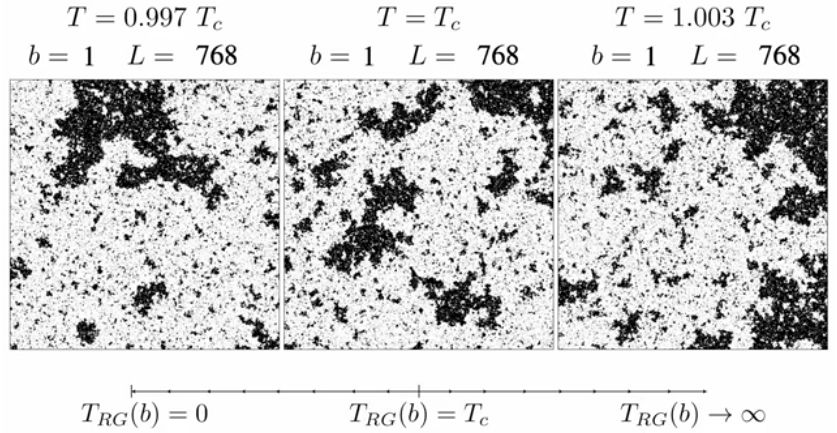
\includegraphics[width=0.8\textwidth]{DouglasAshton1}
	\end{center}
\end{figure}

\begin{figure}[H]
	\caption[Evolving $T=0.997T_c$ after \cite{ashton2012renormalization}]{Evolving $T=0.997T_c$ after \cite{ashton2012renormalization}. The system is strongly coupled, and one colour,in this case white, dominates more and more as we zoom out.}\label{fig:douglas:ashton1}
	\begin{subfigure}[t]{0.3\textwidth}
		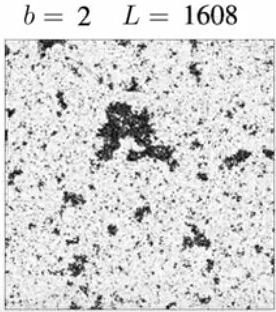
\includegraphics[width=\textwidth]{DouglasAshton1-1}
	\end{subfigure}
	\begin{subfigure}[t]{0.3\textwidth}
		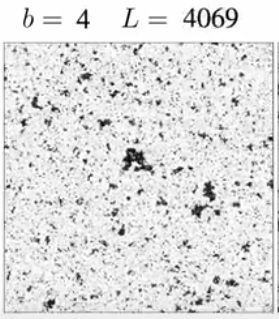
\includegraphics[width=\textwidth]{DouglasAshton1-2}
	\end{subfigure}
	\begin{subfigure}[t]{0.3\textwidth}
		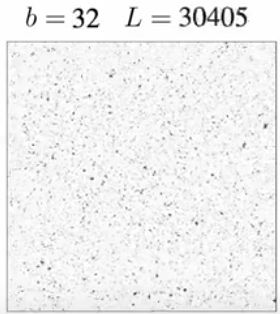
\includegraphics[width=\textwidth]{DouglasAshton1-3}
	\end{subfigure}
\end{figure}

\begin{figure}[H]
	\caption[Evolving $T=1.003T_c$ after \cite{ashton2012renormalization}]{Evolving $T=1.003T_c$ after \cite{ashton2012renormalization}. The coupling is just too weak. As we zoom out, the patches get smaller and smaller, und we end up with something resembling ''snow'' on a TV. Recall that this $T$ and the one in Figure \ref{fig:douglas:ashton1} both looked like the one in the middle of Figure \ref{fig:douglas:ashton} before we zoomed.}
	\begin{subfigure}[t]{0.3\textwidth}
		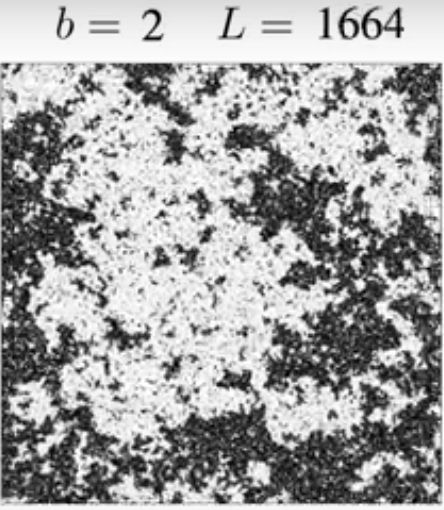
\includegraphics[width=\textwidth]{DouglasAshton2-1}
	\end{subfigure}
	\begin{subfigure}[t]{0.3\textwidth}
		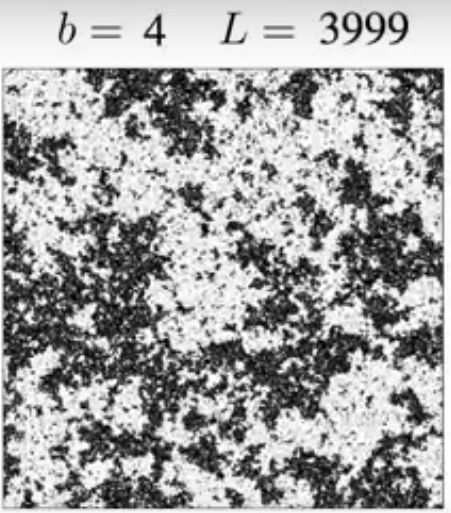
\includegraphics[width=\textwidth]{DouglasAshton2-2}
	\end{subfigure}
	\begin{subfigure}[t]{0.3\textwidth}
		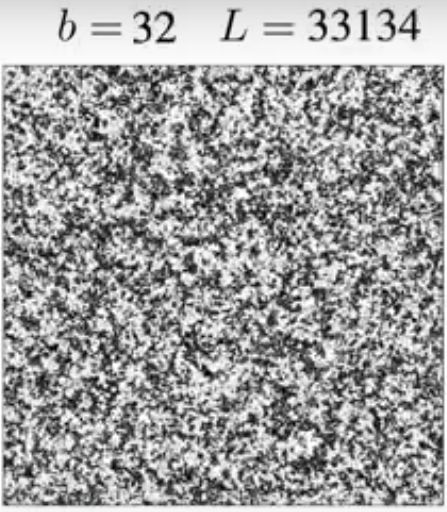
\includegraphics[width=\textwidth]{DouglasAshton2-3}
	\end{subfigure}
\end{figure}

\begin{figure}[H]
	\caption[Evolving $T=T_c$ after \cite{ashton2012renormalization}]{Evolving $T=T_c$ after \cite{ashton2012renormalization}.  little islands shrink, but there are larger islands of correlation that scale down to take their place. There are fluctuations on all scale, in a uniform ''fractal'' pattern. }
	\begin{subfigure}[t]{0.3\textwidth}
		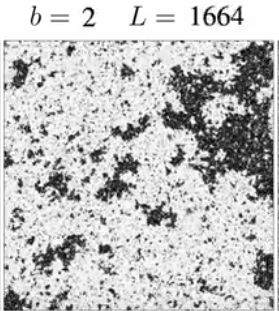
\includegraphics[width=\textwidth]{DouglasAshton3-1}
	\end{subfigure}
	\begin{subfigure}[t]{0.3\textwidth}
		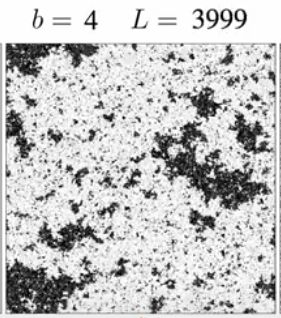
\includegraphics[width=\textwidth]{DouglasAshton3-2}
	\end{subfigure}
	\begin{subfigure}[t]{0.3\textwidth}
		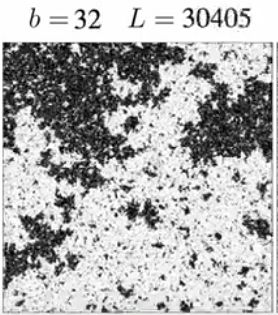
\includegraphics[width=\textwidth]{DouglasAshton3-3}
	\end{subfigure}
\end{figure}

\begin{figure}[H]
	\begin{center}
		\caption[Evolved Ising Model Simulations after \cite{ashton2012renormalization}]{Evolved Ising Model Simulations after \cite{ashton2012renormalization}. A comparison of the three simulations zoomed to the same scale.}
		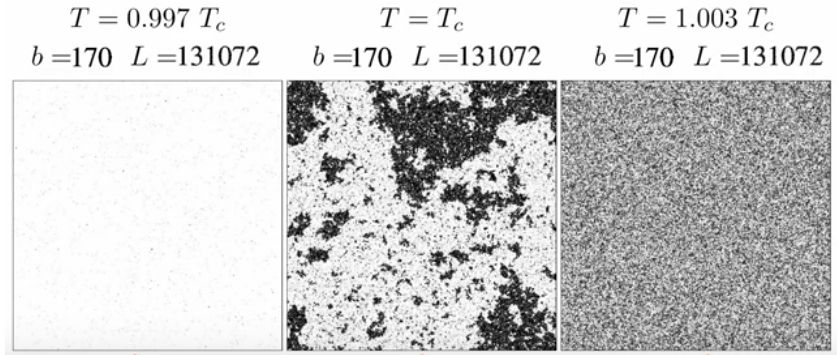
\includegraphics[width=0.8\textwidth]{DouglasAshtonSummary}
	\end{center}
\end{figure}

See also \cite{dedeo2012dynamics}

\section{Krohn-Rhodes Theorem}

\subsection{An Introduction to Group Theory}

Imagine a creature with a set of internal states, and a library of actions that we can perform. E.g., Figure \ref{fig:copy:swap}.

\begin{figure}[H]
	\begin{center}
		\caption[A creature with a set of internal states]{A creature with a set of internal states, and a library of actions that we can perform. Horizontal double arrows represent Swap, single arrows Cycle.}\label{fig:copy:swap}
		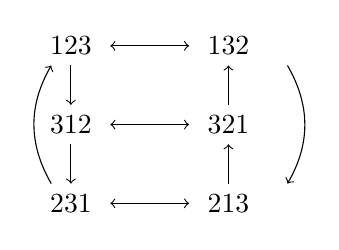
\begin{tikzpicture}
			\draw (1,1) node {231};
			\draw (1,2) node {312};
			\draw (1,3) node {123};
			\draw (3,1) node {213};
			\draw (3,2) node {321};
			\draw (3,3) node {132};
			\draw[->] (1,2.75) -- (1,2.25);
			\draw[->] (1,1.75) -- (1,1.25);
			\path [bend left,->] (0.75,1.25) edge (0.75,2.75);
			\draw[<->] (1.5,3)--(2.5,3);
			\draw[<->] (1.5,2)--(2.5,2);
			\draw[<->] (1.5,1)--(2.5,1);
			\draw[->] (3,2.25) -- (3,2.75);
			\draw[->] (3,1.25) -- (3,1.75);
			\path [bend left,->] (3.75,2.75) edge (3.75,1.25);
		\end{tikzpicture}
	\end{center}
\end{figure}

Figure \ref{fig:coarse:grain:creature} shows a consistent way to coarse-grain the creature, so the coarse-grained state machine is deterministic.

\begin{figure}[H]
	\caption{Coarse Graining the creature}\label{fig:coarse:grain:creature}
	\begin{subfigure}[t]{0.45\textwidth}
		\begin{center}
			\caption{Partitioning into two equivalence classes $A$ and $B$.}
			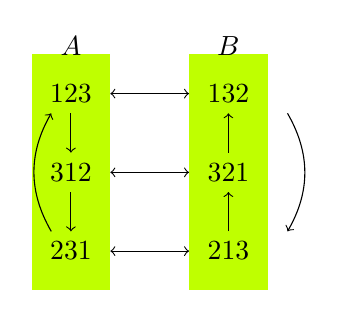
\begin{tikzpicture}
				\fill [lime] (0.5,3.5) rectangle (1.5,0.5);
				\fill [lime] (2.5,3.5) rectangle (3.5,0.5);
				\draw (1,3.6) node {$A$};
				\draw (3,3.6) node {$B$};
				\draw (1,1) node {231};
				\draw (1,2) node {312};
				\draw (1,3) node {123};
				\draw (3,1) node {213};
				\draw (3,2) node {321};
				\draw (3,3) node {132};
				\draw[->] (1,2.75) -- (1,2.25);
				\draw[->] (1,1.75) -- (1,1.25);
				\path [bend left,->] (0.75,1.25) edge (0.75,2.75);
				\draw[<->] (1.5,3)--(2.5,3);
				\draw[<->] (1.5,2)--(2.5,2);
				\draw[<->] (1.5,1)--(2.5,1);
				\draw[->] (3,2.25) -- (3,2.75);
				\draw[->] (3,1.25) -- (3,1.75);
				\path [bend left,->] (3.75,2.75) edge (3.75,1.25);
			\end{tikzpicture}
		\end{center}
	\end{subfigure}
	\hfill
	\begin{subfigure}[t]{0.45\textwidth}
		\caption{Coarse-grained state machine}
		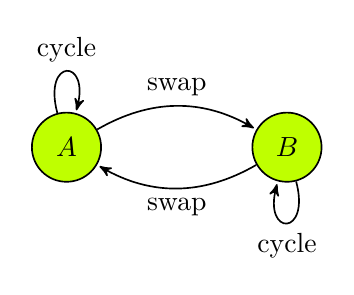
\begin{tikzpicture}[->,>=stealth',shorten >=1pt,auto,node distance=2.8cm,
			semithick]
			\node[state,fill=lime] (A) {$A$};
			\node[state,fill=lime] (B) [right of=A] {$B$};
			\path (A) edge  [bend left]  node {swap} (B);
			\path (B) edge  [bend left]  node {swap} (A);
			\path (A) edge  [loop above] node {cycle} (A);
			\path (B) edge  [loop below] node {cycle} (B);
		\end{tikzpicture}
	\end{subfigure}	
\end{figure}
Note that all sequences are reversible; they form a \textit{group}. It is a consequence of the Jordan–H\''older Theorem--Theorem \ref{thm:JH}--that any two decompositions of a group are isomorphic.

\begin{thm}[Jordan–H\''older]\label{thm:JH}
	Let G be a group, and let $G=G_1 \supset G_2\supset...\supset G_p=\{e\}$ be a normal tower such that each group $G_i/G_{i+1}$ is simple, and $G_i\ne G_{i+1}\forall i$. Then any other tower having the same properties is equivalent to this one.
\end{thm}
\begin{proof}
	\cite{lang02}
\end{proof}
\subsection{Irreversible Computations, Forgetful Computers and the Krohn-Rhodes Theorem }

During the 1960s, Krohn and Rhodes showed that we could also decompose irreversible operations as well.  --semigroup

See \cite{dedeo2011effective,maler2010krohn,rhodes2009applications}

\section{Renormalization in Quantum Electrodynamics}

\subsection{From Quantum Electrodynamics to Plasma Physics }

One of the most important uses of renormalization theory, at least in theoretical physics, is associated with the theory of quantum electrodynamics.
In fact, the person, or the two people,
who first told us
how to use renormalization theory
to understand the quantum theory
of electromagnetism,
how photons and electrons
could interact with each other
in cases where, for example,
electrons could interact,
not just with other photons,
but with electron-positron pairs
that sort of sprung out of a vacuum –
the people who first helped us
understand that
were Murray Gell-Mann,
our very own from Santa Fe Institute,
and Frank Low,
who, in a paper in the 1950s,
talked about quantum electrodynamics
at short distances.
And one of the things they figured out
was how to describe
the following phenomenon.

So, you have some electron–-Figure \ref{fig:Virtual_Pairs}--
in your space, and when you ask what kind of effect does that electron have at a distant point.
One of the things that you have to take into account, at least in quantum electrodynamics, is that even though this vacuum appears to be empty, even though you sort of stipulated that there's nothing between you and the electron, it so turns out in fact, that field of the electron can actually sort of tear
positrons--
positively-charged antielectrons--and electrons out of the vacuum itself.
\begin{figure}[H]
	\begin{center}
		\caption{Virtual Pairs: electrons are shown in blue}\label{fig:Virtual_Pairs}
		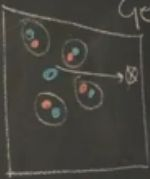
\includegraphics[width=0.6\textwidth]{Virtual_Pairs}
	\end{center}
\end{figure}
So, bizarrely enough,
you get these.
Even though you think
the vacuum is empty,
quantum mechanically it's not,
and so you have
this amazing phenomenon,
where these, what are called
literally ''virtual pairs'',
so you can't actually touch them directly,
you can't sort of nip in
and pull one out,
or maybe you can
if you're fast enough – right? –
But sometimes you haven't
put these in by hand,
and yet they exist.
And what that means in fact
is that the influence
of the electron on that distant point
is modified and modulated
by all of the stuff
that's happening in between.
The closer and closer
you get to the electron,
the less and less those effects conspire
to change the underlying theory,
but what Gell-Mann and Low noticed –
in fact, everybody
was dealing with this problem –
was that the closer
you got to the electron,
the more you sort of dove
into this virtual cloud,
the stronger and stronger
the effects of the electron itself got.
And, in fact, what happened
at very small distances
was that the charge of the electron,
the effect it had on you,
seemed to diverge and become infinite.

So that was a huge problem.
No one knew how to solve it 
And, in the end, they invented
a series of mathematical tools
to help people understand
how they could solve it.

Now, we don't have time to teach you
quantum field theory,
let alone the renormalization problem,
but, beautifully enough,
we do have a sort of toy model
for how this renormalization process works
for the kinds of physics
that Gell-Mann and Low were doing,
and then later, of course, Feynman,
and then a number of other people
who followed in their footsteps.

And in fact what we can do is talk,
not about quantum fluctuations,
which were much harder – right? –
you had to talk about virtual worlds
and all sorts
of philosophically compelling,
but mathematically difficult things.
In fact, it turns out that we can tell
a good part of this story
not in terms of quantum fluctuations,
but in terms of sort of
classical thermal fluctuations.
And in fact you've already seen
an example of thermal fluctuations
when we introduced the Ising model.

As you remember, we had this coupling
parameter, $\beta$, in the Ising model.
The stronger the coupling was,
the more and more the particles
like to align with each other.
They wanted their internal states
to be the same.
So, now, as you decrease
the coupling parameter,
or, in physics language,
as you increase the temperature,
particles had a greater
and greater tolerance
for, instead of both being
in the same state,
for sometimes them to flip.
And you can think of this
as a thermal fluctuation.
The minimal energy configuration is either the particles all pointing up,
or the particles all pointing down,
but instead, if the temperature
is high enough,
you sometimes get these fluctuations,
and if the temperature
is high enough in the Ising model,
those fluctuations can actually
propagate arbitrarily far:
you go through the critical point
and then, in fact, you totally decouple,
and now they seem
totally uncorrelated.

So, what we're going to do now
is tell the story
about the behavior of electrodynamics
in the presence of thermal fluctuation,
not in the presence of these sort of
strange virtual particles,
but in something that you interact with
every day of your life,
although hopefully
only in an intermediate fashion,
because otherwise you would die.
And that is the plasma--Figure \ref{fig:plasma-0}

\begin{figure}[H]
	\begin{center}
		\caption[What is a plasma?]{What is a plasma? A plasma is just a gas 	where the positive nuclei have been separated from the negatively charged electrons.}\label{fig:plasma-0}
		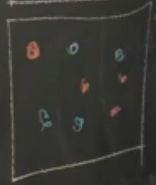
\includegraphics[width=0.6\textwidth]{plasma0}
	\end{center}
\end{figure}

In fact, for example, in the case of the solar wind, you have this gas
that's coming off the Sun, it's being bombarded by photons, the Sun is extremely hot,
and occasionally those photons will rip the electron off an atom, and that electron will fly off.
But the gas is so diffuse, in fact, that it can never really find its old nuclei again.
It can never recondense back together, and so the solar wind is an example of a very diffuse plasma.
On earth we build plasmas all the time.
One of the most extreme cases that we do is when we try to build the tokamak, in other words, when we try to get nuclear fusion going.
To do that, we'll take something like helium or hydrogen, we'll heat it up as hot as we can, separate out the positively charged nuclei from the electrons, and then do some magic and try to get the nuclei to stick together, and that's a whole another story, and it's always 20 years in the future, that solution.

But plasmas exist in all sorts of places in the real world, including, for example,
in the fluorescent lights.
So in that tube you have a very rarefied gas, and what happens is the electric field
produced on either end of that tube, enables the gas to separate out into its constituent positively and negatively charged particles.

So, what we're going to do, our plasma is going to be our virtual background of particles
that occurred in quantum electrodynamics, except now it's much easier, we aren't having to think about how these could be ripped apart from nothing.
Instead, what we're going to assume is that we have some gas, let's say in a box, and the gas is separated into its positive and negatively charged parts.

\subsection{The Thermal Physics of Plasma}

Figure \ref{fig:plasma} shows a plasma, coarse-grained so each space is roughly in electrical equilibrium. This assumes that the particles are well mixed. Assume also that the plasma is in thermal equilibrium (\ref{eq:plasma_thermal}).
\begin{figure}[H]
	\caption{Plasma: each space is roughly in electrical equilibrium}\label{fig:plasma}
	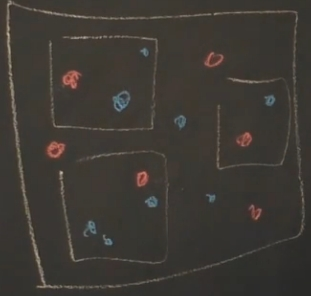
\includegraphics[width=0.9\textwidth]{plasma}
\end{figure}

In thermal equilibrium the number of particles of species $S$ at point $x$ is given by:

\begin{align*}
	n_S(x)=&n_0 e^{- \frac{E(x)}{kT}}  \numberthis \label{eq:plasma_thermal}
\end{align*}

We will assume that the dynamics is controlled by the electrostatic field,  $\Phi$, only.
\begin{align*}
	E(x) =& e_S\Phi\\
	n_S(x)=&n_0 e^{- \frac{e_S\Phi}{kT}} \text{. So the expected numbers of ions  and electrons are}\\
	n_i(x)=&n_0 e^{- \frac{e\Phi}{kT}}\\
	n_e(x)=&n_0 e^{ \frac{e\Phi}{kT}}
\end{align*}
As the temperature goes down, you are less and less likely to find a positively charged particle in a region where there are lots of other positively charged particles. The the positively charged particles will induce a strong electrical field, so adding another particle is unlikely.
\begin{itemize}
	\item As the temperature goes down, you are less and less likely to find a positively charged particle in a region where there are lots of other positively charged particles. The the positively charged particles will induce a strong electrical field, so adding another particle is unlikely. The plasma will be more structured -- +ve balanced by -ve;
	\item at high temperature, may often get transient areas with high charge (dissipate quickly).
\end{itemize}

How does this gas react when we introduce a new test particle? This is analogous to introducing an electron into the quantum vacuum.

\subsection{How does a particle move the plasma?}

In the previous section we saw that the expected numbers of ions  and electrons are given by:
\begin{align*}
	n_i(x)=&n_0 e^{- \frac{e\Phi}{kT}}\\
	n_e(x)=&n_0 e^{ \frac{e\Phi}{kT}}
\end{align*}
Electrons don't like to be too close to each other, but they become more tolerant as the temperature increases. How does this thermal equilibrium interact with an electrical field? We will introduce a test particle.

\begin{figure}[H]
	\begin{center}
		\caption{Introduction of a Test Particle $X$}
		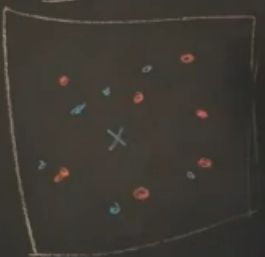
\includegraphics[width=0.6\textwidth]{introduce-test-particle}
	\end{center}
\end{figure}
The electric field potential is given by
\begin{align*}
	\nabla^2 \Phi=& -\frac{\rho}{\epsilon_0}  \text{, so, if the charge $q$ concentrated at a single point}\\
	\Phi =& \frac{q}{4 \pi \epsilon_0 r}
\end{align*}
Now imagine we introduce a small charge $\delta \rho$ into our thermal plasma. If we allow for the movement of charges caused by introducing the extra charge:
\begin{align*}
	\delta \rho =& \underbrace{\delta \rho_{ext}}_\text{Introduced} + \underbrace{e(\delta n_i - \delta n_e)}_\text{Rearrangement of existing charges}.
\end{align*}

We can calculate $\delta n_i - \delta n_e$.
\begin{align*}
	n_i(x)=&n_0 e^{- \frac{e\Phi}{kT}}\\
	=& n_0\big(1 - \frac{e\Phi}{kT} +...\big)\\
	n_e(x)=&n_0 e^{ \frac{e\Phi}{kT}}\\
	=& n_0\big(1 + \frac{e\Phi}{kT} +...\big)
\end{align*}
Whence:
\begin{align*}
	\delta \rho =& \delta \rho_{ext} - \frac{2 e^2 n_0}{kT}\delta \Phi \numberthis \label{eq:delta:rho}
\end{align*}
The reduction in $\delta \rho$ is reduced if the charge of the electron is reduced, or if the temperature increases. Conversely, if the temperature decreases, the test particle can be surrounded by a halo.

\begin{align*}
	\nabla^2 \delta \Phi =& - \frac{1}{\epsilon_0} \big[\delta \rho_{ext} - \frac{2 e^2 n_0}{kT} \delta \Phi\big]
\end{align*}
It can be shown that:
\begin{align*}
	\delta \Phi =& \frac{q}{4 \pi \epsilon_0 r} e^{- \sqrt{2} \frac{r}{\lambda_D}}\text{, where } \numberthis \label{eq:delta_phi}\\
	\lambda_D =& \sqrt{\frac{kT}{w^2 n_0}}
\end{align*}
$\lambda_D$ is known as the ''Debye Length''.

How can we understand the modification of classical electrodynamics that comes from this background of charges?

\begin{figure}[H]
	\begin{center}
		\caption[Effect of background of charge]{Modification of classical electrodynamics that comes from this background of charges. If you get far enough away from charge, its effect is negligible because of screening.}
		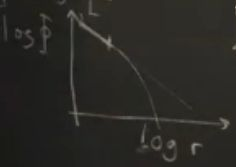
\includegraphics[width=0.8\textwidth]{log-plot}
	\end{center}
\end{figure}

You can think of this as the force becoming weaker as you go further away. The alternative is to rearrange \eqref{eq:delta_phi}, so the charge weakens with distance.
\begin{align*}
	\delta \Phi =& \frac{\overbrace{q e^{- \sqrt{2} \frac{r}{\lambda_D}}}^\text{''Charge''}}{4 \pi \epsilon_0 r} 
\end{align*}
This view is in harmony with the notion of renormalization that we developed in for preceding sections.

\subsection{Charge Renormalization and Feedback}

We can think of \eqref{eq:delta:rho} as renormalizing the charge, which is altered by the field. Think of sticking particle in, then asking how it behaves if we view it as surrounded by boxes of larger and larger scale. We view it as a theory or coarse-graining charge--Figure \ref{fig:coarse_grain_charge}.

\begin{figure}[H]
	\caption{Coarse-graining the Charge, which falls off past the Debye length}\label{fig:coarse_grain_charge}
	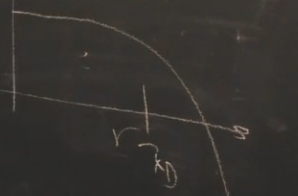
\includegraphics[width=0.9\textwidth]{coarse_grain_charge}
\end{figure}

\begin{itemize}
	\item What is the charge? Actually it depends on the resolution of equipment used to measure! 
	\item At large distances charge disappears. 
	\item Debye length is the scale at which electromagnetic field acts.
	\item For the Solar wind, Debye length is on the scale of metres.
	\item Keep theory the same, and talk about how parameters flow.
	\item Gravitation non-renormalizable. Compare with Ising: higher order coupling get larger and larger.
\end{itemize}

\section{The Future of Renormalization \& Rate Distortion Theory}

When we project, we have some idea what we want.

Utility function.

Rate Distortion Theory --how to balance the need for efficient representation and good representation. Let ${x}$ represent state of World, ${\tilde{x}}$ the state of the brain. The mutual information $I(x,\tilde{x})$ is a measure of how good a job the eye is doing. coarse-graining is $P(\tilde{x}\vert x)$ (soft clustering).

Rate Distortion Theory is about choosing the ''best'' $P(\tilde{x}\vert x)$. We need a distorting=n measure $d(\tilde{x}\vert x)$, the personalty for thinking the world is in state $\vert x$ when it is actually in state $x$ (not symmetric).

\printglossaries

% bibliography go here

\bibliographystyle{unsrt}
\addcontentsline{toc}{section}{Bibliography}
\bibliography{../complexity}


\end{document}
